\documentclass{article}%
\usepackage[T1]{fontenc}%
\usepackage[utf8]{inputenc}%
\usepackage{lmodern}%
\usepackage{textcomp}%
\usepackage{lastpage}%
%
\usepackage{amsmath}%
\usepackage{amssymb}%
\usepackage{amsfonts}%
\usepackage{graphicx}%
\usepackage{hyperref}%
\usepackage{tikz}%
\usepackage{pgfplots}%
\usetikzlibrary{math}%
\title{AFA 2027 - Física\thanks{This exam was solved and automatically generated with gpt-resolve: \url{https://github.com/lgabs/gpt-resolve}}}%
\author{claude{-}opus{-}5{-}5 (solver) + claude{-}opus{-}5{-}5 (judge)}%
\date{October 29, 2026}%
%
\begin{document}%
\normalsize%
\maketitle%
\section*{Questão 49}

\section*{Solução}

\textbf{Critérios de classificação.} Num referencial orientado:
\begin{itemize}
\item \emph{progressivo}: $v>0$ (o espaço cresce); \emph{retrógrado}: $v<0$ (o espaço decresce);
\item \emph{uniforme}: $a=0$ ($|v|$ constante); \emph{acelerado}: $|v|$ cresce, ou seja, $v\cdot a>0$; \emph{retardado}: $|v|$ decresce, ou seja, $v\cdot a<0$.
\end{itemize}
Para não confundir com o instante final $t$, chamo de $\tau$ um instante qualquer, com $0\le\tau\le t$.

\textbf{Partícula A (espaço $\times$ tempo).} O gráfico é um arco de parábola com concavidade para baixo, então o movimento é uniformemente variado com $a<0$. O vértice (máximo de $s$, onde $v=0$) fica num instante $\tau_V<0$. Logo
\[
v(\tau)=a\,(\tau-\tau_V),\qquad \tau-\tau_V>0 \ \text{ e } \ a<0 \;\Rightarrow\; v(\tau)<0 .
\]
\begin{itemize}
\item $v<0$: o espaço diminui de um valor positivo até $s=0$ em $\tau=t$, então o movimento é \textbf{retrógrado};
\item $v<0$ e $a<0$ dão $v\cdot a>0$, então o movimento é \textbf{acelerado}. No gráfico, isso aparece porque a curva fica cada vez mais inclinada, isto é, $|v|$ aumenta com o tempo.
\end{itemize}
Portanto, a alternativa (a) é \textbf{verdadeira}.

\textbf{Partícula B (velocidade $\times$ tempo).} A reta passa pela origem e é crescente: $v(\tau)=k\tau$, com $k=a>0$. Para $0<\tau\le t$, temos $v>0$, então o movimento é \textbf{progressivo}. Também temos $v\cdot a>0$ ($|v|$ cresce), então ele é \textbf{acelerado}. No instante $\tau=0$ a partícula está apenas momentaneamente em repouso, o que não muda a classificação no intervalo.
\begin{itemize}
\item (b) é falsa, porque o movimento de B não é retrógrado;
\item (c) é falsa, porque o movimento de B não é retardado.
\end{itemize}

\textbf{Partícula C (aceleração $\times$ tempo).} De $0$ a $t$, temos $a=0$, então a velocidade é constante, $v=v_0$. O gráfico $a\times\tau$, porém, não informa o valor nem o sinal de $v_0$:
\begin{itemize}
\item se $v_0>0$, o movimento é uniforme e progressivo;
\item se $v_0<0$, o movimento é uniforme e retrógrado;
\item se $v_0=0$, a partícula está em repouso.
\end{itemize}
Assim, o movimento \emph{não} é \emph{necessariamente} progressivo, e a alternativa (d) é \textbf{falsa}.

\textbf{Conclusão.} A única afirmação correta é a (a): no intervalo de $0$ a $t$, a partícula A tem $v<0$ (retrógrado) e $|v|$ crescente, com $v$ e $a$ de mesmo sinal (acelerado).

ANSWER: (A) A é acelerado e retrógrado%
\newpage%
\section*{Questão 50}

\section*{Solução}

\textbf{Hipóteses.} Mola ideal (sem massa), plano sem atrito e resistência do ar desprezível. Assim, a energia mecânica se conserva desde a soltura até o impacto. Pela figura, a linha tracejada horizontal passa pela posição inicial da esfera; logo, entre a soltura e o lançamento a esfera sobe exatamente $h$. Ela deixa o plano com velocidade $v_0$ inclinada de $\theta = 45^\circ$, paralela ao plano.

\textbf{1) Lançamento oblíquo.} O tempo de subida até a altura máxima é $t_s = \dfrac{v_0 \operatorname{sen}\theta}{g}$. Nesse intervalo, o deslocamento horizontal é
\[
d = v_0\cos\theta \cdot t_s = \frac{v_0^2 \operatorname{sen}\theta\cos\theta}{g} = \frac{v_0^2}{2g}\qquad(\theta = 45^\circ).
\]
O enunciado dá $d = 1{,}5\,h$. Portanto
\[
\frac{v_0^2}{2g} = 1{,}5\,h \;\Longrightarrow\; v_0^2 = 3gh \;\Longrightarrow\; \tfrac12 m v_0^2 = 1{,}5\,mgh .
\]

\textbf{2) Conservação da energia (soltura $\to$ lançamento).} A energia elástica é
\[
E_{el} = \tfrac12 k x^2 = \tfrac12\,(100)\,(0{,}20)^2 = 2{,}0\ \text{J}.
\]
Ela se converte em energia potencial gravitacional e energia cinética:
\[
\tfrac12 k x^2 = mgh + \tfrac12 m v_0^2 = mgh + 1{,}5\,mgh = 2{,}5\,mgh
\;\Longrightarrow\; mgh = \frac{2{,}0}{2{,}5} = 0{,}80\ \text{J}.
\]
Como $m = 1{,}0\cdot 10^{-3}$ kg, obtemos $h = 80$ m e $v_0^2 = 3gh = 2400\ \text{m}^2/\text{s}^2$.

\textbf{3) Energia cinética no ponto mais alto.} No topo da parábola só resta a componente horizontal da velocidade, que é constante: $v_x = v_0\cos 45^\circ$, ou seja, $v_x^2 = v_0^2/2$. Então
\[
E_c = \tfrac12 m v_x^2 = \tfrac12\cdot\tfrac12 m v_0^2 = \tfrac12\,(1{,}5\,mgh) = 0{,}75\cdot 0{,}80 = 0{,}60\ \text{J}.
\]
\emph{Verificação:} a energia mecânica no topo é $E_c + mg(h + H_{max})$, com $mgH_{max} = \tfrac12 m (v_0\operatorname{sen}45^\circ)^2 = 0{,}60$ J. O total dá $0{,}60 + 0{,}80 + 0{,}60 = 2{,}0$ J $= E_{el}$, como esperado.

\textbf{4) Aquecimento na colisão.} A esfera para no choque com o bloco. Metade de $E_c$ vira calor sensível da própria esfera:
\[
Q = \tfrac12 E_c = 0{,}30\ \text{J} = m\,c_{Pb}\,\Delta T
\;\Longrightarrow\;
\Delta T = \frac{0{,}30}{(1{,}0\cdot 10^{-3})(125)} = \frac{0{,}30}{0{,}125} = 2{,}4\ ^\circ\text{C}.
\]

\textbf{Conferência.} Unidades: $\text{J}/(\text{kg}\cdot\text{J}/(\text{kg}\,^\circ\text{C})) = {}^\circ\text{C}$. Ordem de grandeza: aquecer 1 g de chumbo em $1\ ^\circ$C exige $0{,}125$ J, e $0{,}30$ J corresponde a $2{,}4\ ^\circ$C, o que é coerente.

Desprezar o ganho de energia potencial no plano seria um erro. Daria $\tfrac12 m v_0^2 = 2{,}0$ J, $E_c = 1{,}0$ J e $\Delta T = 4{,}0\ ^\circ$C, valor que não está entre as alternativas. Os valores $9{,}6$; $4{,}8$ e $1{,}2$ correspondem a $4$, $2$ e $\tfrac12$ vezes o resultado correto. Eles vêm de usar a energia errada (por exemplo, toda a energia cinética de lançamento, $1{,}2$ J, ou esquecer o fator $\tfrac12$).

A alternativa correta é, portanto, a (c).

ANSWER: (C) 2,4%
\newpage%
\section*{Questão 51}

\section*{Solução}

\textbf{Hipóteses.} A mola é ideal e não há forças dissipativas. Sobre a partícula agem apenas o peso $mg$, constante, e a força elástica $k\,x$, onde $x = L - L_0$ é a deformação, com $L_0 = 100$ cm. Logo o sistema é um oscilador harmônico vertical, e seu período é
\[
T = 2\pi\sqrt{\frac{m}{k}} .
\]
O peso só desloca a posição de equilíbrio; ele não altera o período.

\textbf{1) Posição de equilíbrio pelo gráfico.} No MHS a energia cinética é máxima quando a força resultante é nula, isto é, na posição de equilíbrio. Isso acontece porque $\dfrac{dE_c}{dx} = mg - kx$ (teorema da energia cinética), que se anula quando $kx = mg$. Pelo gráfico, o máximo $E_c = 0{,}5$ J ocorre em $L = 110$ cm. Então a deformação estática é
\[
d = 110 - 100 = 10\ \text{cm} = 0{,}10\ \text{m},
\qquad k\,d = m\,g \;\Rightarrow\; \frac{k}{m} = \frac{g}{d} = \frac{10}{0{,}10} = 100\ \text{s}^{-2}.
\]

\textbf{2) Período.}
\[
\omega = \sqrt{\frac{k}{m}} = 10\ \text{rad/s},
\qquad
T = \frac{2\pi}{\omega} = 2\pi\sqrt{\frac{d}{g}} = 2\cdot 3{,}0\cdot\sqrt{\frac{0{,}10}{10}} = 6{,}0\cdot 0{,}10 = 0{,}6\ \text{s}.
\]
Unidades: $\sqrt{\text{m}/(\text{m/s}^2)} = \text{s}$.

\textbf{3) Verificação de consistência com o restante do gráfico.}
\begin{itemize}
\item A partícula parte do repouso em $L = 100$ cm e para de novo em $L = 120$ cm. Os extremos ficam simétricos em relação ao equilíbrio (110 cm), e a amplitude é $A = 0{,}10$ m, como esperado de um MHS.
\item Energia no equilíbrio: $E_{c,\max} = \dfrac{kA^2}{2} \Rightarrow 0{,}5 = \dfrac{k\,(0{,}10)^2}{2} \Rightarrow k = 100$ N/m. Daí $m = \dfrac{k\,d}{g} = \dfrac{100\cdot 0{,}10}{10} = 1{,}0$ kg, e de novo $\dfrac{k}{m} = 100\ \text{s}^{-2}$.
\item Conservação da energia de $L = 100$ cm a $L = 120$ cm: $mg\,(0{,}20) = 1{,}0\cdot 10\cdot 0{,}20 = 2{,}0$ J e $\dfrac{k\,(0{,}20)^2}{2} = \dfrac{100\cdot 0{,}04}{2} = 2{,}0$ J. Os valores conferem.
\item O gráfico é de fato uma parábola, pois $E_c = \dfrac{k}{2}\left[A^2 - (x-d)^2\right]$.
\end{itemize}

\textbf{Ordem de grandeza.} O período não depende da amplitude e fica em décimos de segundo, o que é razoável para uma massa de 1 kg numa mola de 100 N/m. Com $\pi$ exato, $T \approx 0{,}63$ s. Com $\pi = 3{,}0$, fornecido pela prova, $T = 0{,}6$ s.

\textbf{Conclusão.} O máximo da energia cinética marca o equilíbrio, que fica 10 cm abaixo do comprimento natural da mola. Isso dá $k/m = g/d = 100\ \text{s}^{-2}$ e $T = 0{,}6$ s, que é a alternativa (c). As outras alternativas não satisfazem $T = 2\pi\sqrt{d/g}$ com $d = 0{,}10$ m.

ANSWER: (C) 0,6 s%
\newpage%
\section*{Questão 52}

\section*{Solução}

\textbf{1) Condição de rolamento sem escorregamento.}
Quando a roda não escorrega, o ponto dela em contato com o solo tem velocidade nula no instante considerado. Então cada roda gira em torno do ponto de contato, e a velocidade do seu eixo (que é a velocidade do trator) vale
\[
v_{\text{eixo}} = \omega R .
\]
As duas rodas estão presas ao mesmo chassi rígido, por isso os eixos dianteiro e traseiro têm a mesma velocidade $v(t)$ em todo instante, inclusive durante a aceleração e a frenagem:
\[
v(t) = \omega_D(t)\,R_D = \omega_T(t)\,R_T .
\]

\textbf{2) Relação entre as velocidades angulares.}
Pelo enunciado, $R_T = 2R_D$. Daí
\[
\omega_D(t) = \frac{v(t)}{R_D}, \qquad \omega_T(t) = \frac{v(t)}{2R_D} = \frac{\omega_D(t)}{2}
\quad\Longrightarrow\quad \omega_D(t) = 2\,\omega_T(t)\ \text{ para todo } t .
\]
Faz sentido fisicamente: no mesmo intervalo de tempo as duas rodas percorrem a mesma distância no solo. A roda menor tem metade do perímetro, então precisa dar o dobro de voltas.

\textbf{3) Forma dos gráficos.}
Como $R_D$ e $R_T$ são constantes, $\omega_D$ e $\omega_T$ são proporcionais a $v(t)$. Os gráficos $\omega\times t$ têm, portanto, a mesma forma trapezoidal do gráfico $v\times t$ e os mesmos instantes $0$, $t_1$, $t_2$ e $t_3$:
\begin{itemize}
\item de $0$ a $t_1$: as duas crescem linearmente a partir de zero, com acelerações angulares $\alpha = a/R$, e portanto $\alpha_D = 2\alpha_T$;
\item de $t_1$ a $t_2$: as duas ficam constantes. Chamando $\omega \equiv \omega_T = \dfrac{v}{R_T}$, temos $\omega_D = \dfrac{v}{R_D} = 2\omega$;
\item de $t_2$ a $t_3$: as duas decrescem linearmente e chegam a zero juntas em $t_3$.
\end{itemize}
Conferência das unidades: $\omega = v/R$ tem unidade $(\text{m/s})/\text{m} = \text{rad/s}$.

\textbf{4) Análise das alternativas.}
\begin{itemize}
\item (a) Põe $\omega_T = 2\omega_D$, ou seja, inverte a relação: a roda maior estaria girando mais rápido. Incorreta.
\item (b) $\omega_D = \omega_T$ só valeria se $R_D = R_T$. Incorreta.
\item (c) Os patamares $\omega$ e $\omega/2$ estão na razão certa, mas $\omega_T$ está no patamar maior, o que de novo dá $\omega_T = 2\omega_D$. Incorreta.
\item (d) Mostra $\omega_D$ com patamar $2\omega$ e $\omega_T$ com patamar $\omega$, os dois trapezoidais, com os mesmos instantes $t_1$, $t_2$, $t_3$. Isso corresponde exatamente a $\omega_D = 2\omega_T$. \textbf{Correta.}
\end{itemize}

ANSWER: (D) $\omega_D = 2\,\omega_T$; os dois gráficos são trapézios com os mesmos instantes $t_1$, $t_2$, $t_3$, e o de $\omega_D$ tem o patamar mais alto ($2\omega$ contra $\omega$).%
\newpage%
\section*{q53_solution}%
Solution has invalid LaTeX, see q53\_solution.txt.%
\newpage%
\section*{q54_solution}%
Solution has invalid LaTeX, see q54\_solution.txt.%
\newpage%
\section*{Questão 55}

\section*{Solução}

\textbf{Hipóteses.} A partícula é tratada como ponto material e parte do repouso no topo. A calha é lisa, então não há atrito. A resistência do ar é desprezada. Seja $\beta$ o ângulo da calha com a horizontal. O enunciado garante que $\beta$ não muda com o aquecimento. Seja $L_0$ o comprimento da calha percorrido pela partícula, do topo até a base.

\textbf{1) Aceleração ao longo da calha.} Sobre a partícula atuam o peso $mg$ e a normal $N$, perpendicular à calha. Aplicando a 2.ª lei de Newton na direção da calha:
\[
mg\,\text{sen}\,\beta = m a \quad\Longrightarrow\quad a = g\,\text{sen}\,\beta .
\]
A aceleração é constante e depende apenas de $g$ e de $\beta$. Logo ela é a mesma antes e depois do aquecimento, e não depende de $\alpha$ nem do comprimento da calha.

\textbf{2) Tempo de descida (MUV a partir do repouso).}
\[
L_0 = \frac{a\,t^2}{2} \quad\Longrightarrow\quad t = \sqrt{\frac{2L_0}{g\,\text{sen}\,\beta}}\,, \qquad\text{ou seja,}\qquad t \propto \sqrt{L} .
\]

\textbf{3) Dilatação linear da calha.} A calha é homogênea e $\alpha$ é constante. Portanto, após a variação de temperatura $\Delta\theta$, todo o seu comprimento passa a ser
\[
L = L_0\,(1+\alpha\,\Delta\theta).
\]
A altura do topo também aumenta, na mesma proporção, porque a inclinação não muda. Isso já está incluído no novo comprimento $L$.

\textbf{4) Novo tempo.} A aceleração $a = g\,\text{sen}\,\beta$ é a mesma. Então:
\[
t' = \sqrt{\frac{2L}{g\,\text{sen}\,\beta}} = \sqrt{\frac{2L_0(1+\alpha\,\Delta\theta)}{g\,\text{sen}\,\beta}}
\quad\Longrightarrow\quad
\frac{t'}{t} = \sqrt{\frac{L}{L_0}} = (1+\alpha\,\Delta\theta)^{1/2},
\]
\[
\boxed{t' = t\,(1+\alpha\,\Delta\theta)^{1/2}} .
\]

\textbf{Verificações.}
\begin{itemize}
\item \emph{Dimensão:} $\alpha$ é dado em ${}^\circ\text{C}^{-1}$, logo $\alpha\,\Delta\theta$ é adimensional e $t'$ tem unidade de tempo.
\item \emph{Caso particular:} se $\Delta\theta = 0$, obtemos $t' = t$, como esperado.
\item \emph{Sentido físico:} para $\Delta\theta > 0$, temos $t' > t$, pois a partícula percorre uma calha maior com a mesma aceleração.
\item \emph{Ordem de grandeza:} para um metal, $\alpha \sim 10^{-5}\ {}^\circ\text{C}^{-1}$. Com $\Delta\theta \sim 10^{2}\ {}^\circ\text{C}$, vem $\alpha\,\Delta\theta \sim 10^{-3}$ e $t' \approx t\left(1 + \tfrac{\alpha\,\Delta\theta}{2}\right)$, um aumento de cerca de $0{,}05\%$.
\end{itemize}

\textbf{Análise das alternativas.}
\begin{itemize}
\item (a) Para $\Delta\theta \to 0$, daria $t' \to 0$, o que é absurdo.
\item (c) Valeria se o tempo fosse proporcional ao comprimento ($t \propto L$), o que ocorreria em movimento uniforme.
\item (d) Corresponderia a $t \propto L^2$.
\end{itemize}
Nenhuma dessas relações vale para um MUV que parte do repouso, no qual $t \propto \sqrt{L}$. Portanto a correta é a alternativa (b).

ANSWER: (B) $t\cdot(1+\alpha\cdot\Delta\theta)^{1/2}$%
\newpage%
\section*{Questão 56}

\section*{Solução}

\textbf{1) Velocidade da partícula (filtro de velocidades).}
Como a gravidade e a resistência do ar são desprezadas, sobre a partícula de carga $q$ atuam só a força elétrica e a força magnética (força de Lorentz):
\[
\vec F = q\vec E + q\,\vec v\times\vec B .
\]
A velocidade é constante, então pela 1ª lei de Newton a força resultante é nula:
\[
q\vec E + q\,\vec v\times\vec B = \vec 0 \quad\Longrightarrow\quad \vec v\times\vec B = -\vec E .
\]
Por isso a força magnética precisa ter o mesmo módulo e o sentido oposto ao da força elétrica. Os campos são perpendiculares entre si. Essa é a configuração clássica do \emph{seletor de velocidades}, na qual a velocidade é perpendicular tanto a $\vec E$ quanto a $\vec B$; assim $\operatorname{sen}\theta = \operatorname{sen}90^\circ = 1$ e
\[
|q|\,E = |q|\,v\,B \quad\Longrightarrow\quad v=\frac{E}{B}=\frac{4{,}0\ \text{N/C}}{2{,}0\cdot 10^{-1}\ \text{T}} = 20\ \text{m/s}.
\]
Unidades: $\dfrac{\text{N/C}}{\text{T}}=\dfrac{\text{N/C}}{\text{N}\cdot\text{s}/(\text{C}\cdot\text{m})}=\text{m/s}$. Com $\vec v\perp\vec E$, a força elétrica não realiza trabalho, o que é coerente com a velocidade constante. O resultado também não depende da carga nem da massa.

(Se $\vec v$ tivesse uma componente paralela a $\vec B$, essa componente não geraria força e o módulo de $v$ ficaria indeterminado. Por isso o enunciado pressupõe a configuração do seletor, com $\vec v \perp \vec E$ e $\vec v\perp\vec B$.)

\textbf{2) Velocidade da imagem no espelho plano.}
No espelho plano, a imagem é simétrica ao objeto em relação ao plano do espelho. Em cada instante, a distância da imagem ao espelho é igual à distância da partícula ao espelho:
\[
d_{\text{img}}(t)=d_{\text{obj}}(t)\quad\Longrightarrow\quad \left|\frac{\mathrm{d}d_{\text{img}}}{\mathrm{d}t}\right| = \left|\frac{\mathrm{d}d_{\text{obj}}}{\mathrm{d}t}\right| .
\]
A trajetória da partícula é perpendicular ao espelho. Assim, toda a sua velocidade, $20\ \text{m/s}$, serve para aproximá-la do espelho, e $d_{\text{obj}}$ diminui a $20\ \text{m/s}$. Logo, a imagem se aproxima do espelho, que está fixo, com
\[
v_{\text{img}} = v = 20\ \text{m/s}.
\]

\textbf{3) Conferência das alternativas.}
O valor $40\ \text{m/s}$ seria a velocidade da imagem \emph{em relação à partícula} ($v+v=2v$), e não em relação ao espelho, como pede o enunciado. Os valores $10$ e $80\ \text{m/s}$ não correspondem a nenhuma relação física da situação. Portanto, a alternativa correta é a (b).

ANSWER: (B) 20 m/s
%
\newpage%
\section*{Questão 57}

\section*{Solução}

\textbf{Hipóteses.} O chuveiro funciona em regime permanente, ligado à mesma tensão $U$ e com a mesma resistência $R$. Como a resistividade não depende da temperatura e nada foi alterado na parte elétrica, a potência dissipada
\[
P=\frac{U^2}{R}
\]
é a mesma nas duas situações. Também supomos que toda essa potência (ou ao menos uma fração constante dela) passa para a água, cuja densidade $\rho$ e cujo calor específico $c$ são constantes.

\textbf{Balanço de energia.} Num intervalo $\Delta t$, passa pelo chuveiro a massa $\Delta m=\rho\,\Phi\,\Delta t$, em que $\Phi$ é a vazão volumétrica. Essa massa é aquecida de $\Delta\theta$, logo
\[
P\,\Delta t=\Delta m\,c\,\Delta\theta=\rho\,\Phi\,\Delta t\,c\,\Delta\theta
\quad\Longrightarrow\quad
P=\rho\,c\,\Phi\,\Delta\theta .
\]
Como $P$, $\rho$ e $c$ são constantes, o produto $\Phi\,\Delta\theta$ também é constante: \emph{a elevação de temperatura é inversamente proporcional à vazão}.

\textbf{Cálculo.}
\begin{itemize}
\item Situação 1: $\Phi_1=182\ \text{mL/s}$ e $\Delta\theta_1=31-11=20\ ^\circ\text{C}$.
\item Situação 2: $\Phi_2=130\ \text{mL/s}$ e $\Delta\theta_2=\ ?$
\end{itemize}
\[
\Phi_1\,\Delta\theta_1=\Phi_2\,\Delta\theta_2
\;\Longrightarrow\;
\Delta\theta_2=\frac{182}{130}\cdot 20=1{,}4\cdot 20=28\ ^\circ\text{C}.
\]
Portanto, a temperatura de saída da água é
\[
\theta_2=11+28=39\ ^\circ\text{C}.
\]

\textbf{Conferência.} Ao reduzir a vazão, a temperatura sobe ($39>31$), como era de se esperar. As unidades de vazão aparecem só como razão, então não é preciso convertê-las. Ordem de grandeza: com $\rho c\approx 4{,}2\ \text{J/(mL}\cdot{}^\circ\text{C)}$, temos $P\approx 4{,}2\cdot182\cdot20\approx 15\ \text{kW}$. É uma potência alta, mas da mesma ordem dos chuveiros elétricos potentes, o que confirma que o resultado é plausível. Esse valor só serve de conferência e não é necessário para a resposta.

\textbf{Por que a alternativa (b).} O produto vazão $\times$ elevação de temperatura não muda, então $\Delta\theta_2=28\ ^\circ\text{C}$ e a água sai a $39\ ^\circ\text{C}$. As outras alternativas ($38$, $40$ e $41\ ^\circ\text{C}$) não respeitam essa proporção inversa.

ANSWER: (B) 39%
\newpage%
\section*{Questão 58}

\section*{Solução}

\textbf{Hipóteses.} A barra é rígida, homogênea e está em equilíbrio estático, na iminência de escorregar no apoio $C$. Pela figura, o fio está preso ao teto à esquerda de $A$; logo ele puxa $A$ para cima e para a esquerda, formando o ângulo $\theta$ com a vertical. O campo $\vec B$ é uniforme e aponta para dentro da folha.

\textbf{1) Força magnética.} Num condutor retilíneo, $\vec F_m = i\,\vec L\times\vec B$. Com a corrente de $C$ para $A$, $\vec L$ aponta para a esquerda ($-\hat x$) e $\vec B=-B\,\hat z$. Então
\[
\vec F_m = iLB\,(-\hat x)\times(-\hat z)=iLB\,(\hat x\times\hat z)=-BiL\,\hat y .
\]
A força magnética aponta \emph{para baixo} e vale $BiL$. A barra é homogênea e o campo é uniforme, então essa força se distribui igualmente ao longo da barra e sua resultante atua no ponto médio, assim como o peso. Vamos chamar de carga vertical total
\[
W = mg + BiL .
\]

\textbf{2) Forças na barra.}
\begin{itemize}
\item Em $A$, a tração tem componentes $T\cos\theta$ (para cima) e $T\,\text{sen}\,\theta$ (para a esquerda).
\item No ponto médio atua $W$, para baixo.
\item Em $C$ atuam a normal $N$ (para cima) e o atrito estático $f$. Como o fio tende a arrastar a barra para a esquerda, o atrito em $C$ aponta para a direita.
\end{itemize}

\textbf{3) Equilíbrio de translação.}
\[
\text{horizontal: } f = T\,\text{sen}\,\theta, \qquad \text{vertical: } T\cos\theta + N = mg+BiL .
\]

\textbf{4) Iminência de movimento.} O atrito estático atinge seu valor máximo: $f=\mu N$. Então $N=\dfrac{T\,\text{sen}\,\theta}{\mu}$. Substituindo na equação vertical:
\[
T\cos\theta+\frac{T\,\text{sen}\,\theta}{\mu}=mg+BiL
\;\Longrightarrow\;
T\,\frac{\mu\cos\theta+\text{sen}\,\theta}{\mu}=mg+BiL
\;\Longrightarrow\;
\boxed{T=\frac{\mu}{\mu\cos\theta+\text{sen}\,\theta}\,(mg+BiL)}
\]

\textbf{5) Verificação pelo equilíbrio de rotação.} Tomando momentos em relação a $A$:
\[
N\,L = W\,\frac{L}{2} \;\Rightarrow\; N=\frac{W}{2} \;\Rightarrow\; T\cos\theta=\frac{W}{2},
\qquad f=T\,\text{sen}\,\theta=\frac{W}{2}\,\text{tg}\,\theta .
\]
Logo a iminência ($f=\mu N$) só ocorre se $\mu=\text{tg}\,\theta$. Substituindo $\mu=\text{tg}\,\theta$ no resultado do item 4:
\[
T=\frac{\text{tg}\,\theta}{\text{tg}\,\theta\cos\theta+\text{sen}\,\theta}\,W=\frac{\text{tg}\,\theta}{2\,\text{sen}\,\theta}\,W=\frac{W}{2\cos\theta}.
\]
Isso coincide com o valor obtido pelos momentos, então o resultado é coerente. Unidades: $\mu$ e as funções trigonométricas são adimensionais, e $mg$ e $BiL$ são forças, logo $[T]=\text{N}$. Caso particular: sem corrente ($i=0$), sobra apenas o peso, como esperado.

\textbf{6) Análise das alternativas.}
\begin{itemize}
\item As alternativas (a) e (d) contêm $(mg-BiL)$, mas a força magnética aponta para baixo e se \emph{soma} ao peso. Ambas estão descartadas.
\item A alternativa (b) daria $T=\dfrac{\mu W}{2\cos\theta}$. Como $T=\dfrac{W}{2\cos\theta}$, ela só valeria se $\mu=1$, o que não acontece em geral.
\item A alternativa (c) é exatamente a expressão deduzida a partir do equilíbrio na iminência de deslizamento.
\end{itemize}

ANSWER: (C) $T=\dfrac{\mu}{\mu\cos\theta+\text{sen}\,\theta}\,(mg+BiL)$%
\newpage%
\section*{Questão 59}

\section*{Solução}

\textbf{1. Conservação do momento linear.} Os dois fótons têm momentos de mesmo módulo e sentidos opostos, então o momento total depois da aniquilação é nulo. Como o momento se conserva, o par elétron--pósitron também tinha momento total nulo: o laboratório é o referencial do centro de massa.

Para um fóton, $E = pc$. Se os módulos dos momentos são iguais, as energias também são:
\[
E_1 = E_2 = E_f .
\]

\textbf{2. Conservação da energia (relativística).} Seja $K$ a energia cinética total do par antes da aniquilação. Então
\[
2E_f = m_e c^2 + m_p c^2 + K = 2mc^2 + K, \qquad m = m_e = m_p = 9{,}0\cdot 10^{-31}\ \text{kg}.
\]
Como $K \geq 0$, a energia de cada fóton é \emph{mínima} quando $K = 0$, isto é, quando as partículas estão praticamente em repouso. Nesse caso apenas as massas de repouso viram energia, como diz o enunciado:
\[
E_{f,\min} = mc^2 = 9{,}0\cdot 10^{-31}\cdot\left(3{,}0\cdot 10^{8}\right)^2 = 8{,}1\cdot 10^{-14}\ \text{J}.
\]
(Isso dá cerca de $0{,}5\ \text{MeV}$, que é o valor conhecido para os fótons da PET.)

\textbf{3. Relação de Planck.} Como $E = hf$:
\[
f_{\min} = \frac{mc^2}{h} = \frac{8{,}1\cdot 10^{-14}}{6{,}6\cdot 10^{-34}} \approx 1{,}2\cdot 10^{20}\ \text{Hz}.
\]
Unidades: $\dfrac{\text{J}}{\text{J}\cdot\text{s}} = \text{s}^{-1} = \text{Hz}$.

\textbf{4. Ordem de grandeza.} Escrevemos $f_{\min} = 1{,}2\cdot 10^{20}\ \text{Hz}$. Como $1{,}2 < \sqrt{10} \approx 3{,}16$, a ordem de grandeza é $10^{20}\ \text{Hz}$. Essa frequência está na faixa dos raios gama, o que é coerente com o fenômeno.

\textbf{Análise das alternativas.} As alternativas (a) $10^{12}$ e (b) $10^{15}$ correspondem a infravermelho e ultravioleta: são energias muitas ordens de grandeza menores que $mc^2$. A alternativa (d) $10^{24}$ exigiria cada fóton com energia cerca de $10^4$ vezes maior que a energia de repouso do elétron. Isso contraria a hipótese de frequência mínima, que corresponde a $K = 0$. Só a alternativa (c) é compatível com $f_{\min} \approx 1{,}2\cdot 10^{20}\ \text{Hz}$.

ANSWER: (C) $10^{20}$%
\newpage%
\section*{Questão 60}

\section*{Solução}

\textbf{Hipóteses e leis.} As cargas são puntiformes, estão fixas e há um único meio, com constante $k$. Seja $L$ o lado do triângulo. Pela lei de Coulomb, a força que $Q_i$ exerce sobre $Q_B$ tem módulo
\[
F_{iB}=\frac{k\,|Q_i|\,|Q_B|}{L^2}
\]
e atua na reta que une as duas cargas. Ela é de repulsão se os sinais são iguais e de atração se são opostos. Pelo princípio da superposição, $\vec F=\vec F_{AB}+\vec F_{CB}$.

\begin{center}
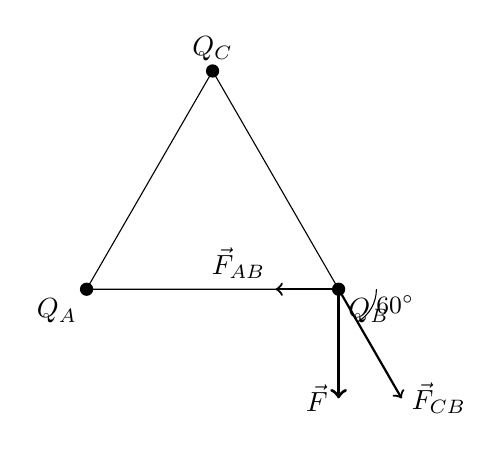
\begin{tikzpicture}[scale=1.6]
\coordinate (A) at (0,0); \coordinate (B) at (2,0); \coordinate (C) at (1,1.732);
\draw (A)--(B)--(C)--cycle;
\fill (A) circle (1.5pt) node[below left]{$Q_A$};
\fill (B) circle (1.5pt) node[below right]{$Q_B$};
\fill (C) circle (1.5pt) node[above]{$Q_C$};
\draw[->,thick] (B)--++(0.5,-0.866) node[right]{$\vec F_{CB}$};
\draw[->,thick] (B)--++(-0.5,0) node[above left]{$\vec F_{AB}$};
\draw[->,very thick] (B)--++(0,-0.866) node[left]{$\vec F$};
\draw (B)++(0.3,0) arc (0:-60:0.3); \node at (2.45,-0.12) {\small $60^\circ$};
\end{tikzpicture}
\end{center}

\textbf{Decomposição.} Tome o eixo $x$ de $A$ para $B$ e o eixo $y$ vertical para cima. Pela figura da prova, a força resultante sobre $Q_B$ é $\vec F=-F\,\hat y$, ou seja, perpendicular a $AB$ e voltada para baixo.
\begin{itemize}
\item $\vec F_{AB}$ age ao longo de $AB$. Portanto é horizontal e não tem componente $y$.
\item $\vec F_{CB}$ age ao longo de $CB$, que forma $60^\circ$ com a horizontal. O unitário que vai de $C$ para $B$ é $\hat u=(\cos 60^\circ,\,-\text{sen}\,60^\circ)=\left(\tfrac12,\,-\tfrac{\sqrt3}{2}\right)$.
\end{itemize}

\textbf{(i) Componente vertical.} Só $\vec F_{CB}$ tem componente $y$, e ela precisa ser negativa. Logo $\vec F_{CB}$ tem o sentido de $\hat u$: a força afasta $B$ de $C$, isto é, há repulsão. Então $Q_C$ tem o mesmo sinal de $Q_B$, ou seja, $Q_C<0$.

\textbf{(ii) Componente horizontal.} A componente $x$ de $\vec F_{CB}$ vale $F_{CB}\cos 60^\circ=F_{CB}/2$ e aponta no sentido $+x$. Como a resultante não tem componente horizontal, $\vec F_{AB}$ tem de apontar para $-x$, isto é, de $B$ para $A$. Trata-se de atração, logo $Q_A$ tem sinal oposto ao de $Q_B$ e $Q_A=+1\ \mu\text{C}$. Além disso,
\[
F_{AB}=F_{CB}\cos 60^\circ
\;\Longrightarrow\;
\frac{k|Q_A||Q_B|}{L^2}=\frac12\,\frac{k|Q_C||Q_B|}{L^2}
\;\Longrightarrow\;
|Q_C|=2|Q_A|=2\ \mu\text{C}.
\]
Logo $Q_C=-2\ \mu\text{C}$. Os fatores $k$, $L$ e $|Q_B|$ se cancelam, e por isso o enunciado não precisa fornecê-los.

\textbf{Verificação.} Com $Q_A=+1\ \mu\text{C}$ e $Q_C=-2\ \mu\text{C}$, as componentes horizontais se anulam: $F_{AB}-\tfrac12F_{CB}=0$. A resultante vale $F=F_{CB}\,\text{sen}\,60^\circ=\tfrac{\sqrt3}{2}F_{CB}$ e aponta para baixo, como na figura.

\textbf{Soma das cargas.}
\[
Q_A+Q_B+Q_C=(+1)+(-3)+(-2)=-4{,}0\ \mu\text{C}.
\]

\textbf{Por que as outras alternativas estão erradas.} Com $Q_C>0$ haveria atração entre $B$ e $C$, e $\vec F_{CB}$ teria componente para cima, o que contradiz a figura. Isso exclui, por exemplo, $Q_A=+1$ e $Q_C=+2$ (soma $0$, alternativa c). A alternativa b ($-1{,}5$) aparece quando se inverte a projeção e se escreve $|Q_C|=|Q_A|/2$. A alternativa d ($+6{,}0$) é incompatível com os sinais obtidos em (i) e (ii). Portanto, a alternativa correta é a (A).

ANSWER: (A) $-4{,}0\ \mu\text{C}$%
\newpage%
\section*{Questão 61}

\section*{Solução}

\textbf{Hipóteses.} O múon é uma partícula livre e relativística. Todas as grandezas ($K$, $p$, $\lambda$) são medidas no referencial da Terra. O comprimento de onda de De Broglie é
\[
\lambda=\frac{h}{p},
\]
em que $p$ é o módulo do momento linear \emph{relativístico}. Como os múons dos raios cósmicos têm velocidades próximas de $c$, não se pode usar $p=\sqrt{2m_0K}$, que só vale para $v\ll c$.

\textbf{1) Energia total.} A energia total do múon é a energia de repouso mais a cinética:
\[
E = m_0c^2 + K .
\]

\textbf{2) Relação energia--momento.} Para uma partícula livre (invariante relativístico):
\[
E^2 = p^2c^2 + m_0^2c^4 .
\]
Substituindo $E$:
\[
\left(m_0c^2+K\right)^2 = p^2c^2 + m_0^2c^4
\;\Longrightarrow\;
m_0^2c^4 + 2m_0c^2K + K^2 = p^2c^2 + m_0^2c^4 ,
\]
\[
p^2c^2 = K^2 + 2m_0c^2K
\;\Longrightarrow\;
p=\sqrt{\frac{K^2}{c^2}+2m_0K}.
\]

\textbf{3) Comprimento de onda.}
\[
\boxed{\lambda=\frac{h}{p}=\frac{h}{\sqrt{2m_0K+\dfrac{K^2}{c^2}}}}
\]

\textbf{Verificações.}
\begin{itemize}
\item \emph{Unidades:} $[m_0K]=\text{kg}^2\,\text{m}^2/\text{s}^2=[p^2]$ e $[K^2/c^2]=\text{J}^2\,\text{s}^2/\text{m}^2=[p^2]$. Logo, o radicando tem dimensão de momento ao quadrado e $\lambda$ sai em metros.
\item \emph{Limite clássico} ($K\ll m_0c^2$): $K^2/c^2\ll 2m_0K$, e então $\lambda\approx h/\sqrt{2m_0K}$, que é a expressão newtoniana.
\item \emph{Limite ultrarrelativístico} ($K\gg m_0c^2$): $\lambda\approx hc/K$, como para um fóton de energia $K$.
\end{itemize}

\textbf{Análise das alternativas.}
\begin{itemize}
\item (c) e (d) somam $K/c$, que tem dimensão de momento, com $2m_0K$, que tem dimensão de momento ao quadrado. São dimensionalmente inconsistentes.
\item (b) tem o sinal errado: o radicando $K^2/c^2-2m_0K$ é negativo para $K<2m_0c^2$, o que inclui todo o regime clássico.
\item (a) coincide com o resultado deduzido e passa nas verificações acima.
\end{itemize}

ANSWER: (A) $\lambda=\dfrac{h}{\sqrt{2m_0K+\dfrac{K^2}{c^2}}}$%
\newpage%
\section*{Questão 62}

\section*{Solução}

\textbf{Hipóteses e convenção.} Os espelhos são esféricos e operam nas condições de Gauss (raios paraxiais). Por isso valem a equação dos pontos conjugados e a do aumento linear:
\[
\frac{1}{f}=\frac{1}{p}+\frac{1}{p'},\qquad A=\frac{i}{o}=-\frac{p'}{p},
\]
com $p>0$ para objeto real, $p'>0$ para imagem real (diante do espelho), $f=+\dfrac{R}{2}$ no côncavo e $f=-\dfrac{R}{2}$ no convexo. Os espelhos estão frente a frente, com os vértices separados por $2R$.

\textbf{1.ª reflexão (espelho côncavo).} Temos $p_1=0{,}75\,R=\dfrac{3R}{4}$ e $f_1=\dfrac{R}{2}$. Então
\[
\frac{1}{p_1'}=\frac{2}{R}-\frac{4}{3R}=\frac{2}{3R}\quad\Longrightarrow\quad p_1'=1{,}5\,R>0 .
\]
A imagem $I_1$ é \emph{real}, fica a $1{,}5\,R$ do côncavo e tem aumento
\[
A_1=-\frac{p_1'}{p_1}=-\frac{1{,}5\,R}{0{,}75\,R}=-2 .
\]
Logo $I_1$ é invertida e tem o dobro da altura do objeto. Isso é coerente com o objeto estar entre o foco ($0{,}5\,R$) e o centro de curvatura ($R$).

\textbf{2.ª reflexão (espelho convexo).} Como $1{,}5\,R<2R$, a imagem $I_1$ se forma \emph{entre} os espelhos. Os raios convergem em $I_1$ e depois divergem até o convexo. Portanto $I_1$ funciona como \emph{objeto real} para o convexo, à distância
\[
p_2=2R-1{,}5\,R=0{,}5\,R .
\]
Com $f_2=-\dfrac{R}{2}$:
\[
\frac{1}{p_2'}=-\frac{2}{R}-\frac{2}{R}=-\frac{4}{R}\quad\Longrightarrow\quad p_2'=-\frac{R}{4}<0 .
\]
A imagem final $I_2$ é \emph{virtual}: fica $0{,}25\,R$ atrás do espelho convexo, como sempre ocorre num convexo com objeto real. O aumento é
\[
A_2=-\frac{p_2'}{p_2}=-\frac{-R/4}{R/2}=+\frac{1}{2}.
\]
Logo $I_2$ é \emph{direita em relação a $I_1$} e tem \emph{metade da altura de $I_1$}.

\textbf{Em relação ao objeto.} O aumento total é
\[
A=A_1A_2=(-2)\cdot\frac{1}{2}=-1 .
\]
Se o objeto tem altura $o$, então $i_1=-2o$ e $i_2=\tfrac12\,i_1=-o$. A imagem final é \emph{invertida em relação ao objeto} e do \emph{mesmo tamanho} dele.

\textbf{Análise das alternativas.}
\begin{itemize}
\item[a)] Falsa. A imagem é virtual e direita em relação a $I_1$, mas tem a mesma altura do objeto ($|A|=1$), não metade.
\item[b)] Falsa. A imagem é virtual, não real.
\item[c)] Falsa. A imagem é virtual, e seu tamanho é metade do de $I_1$, não igual.
\item[d)] Verdadeira. A imagem é virtual ($p_2'<0$), invertida em relação ao objeto ($A=-1$) e tem metade da altura da imagem do côncavo ($A_2=\tfrac12$).
\end{itemize}

ANSWER: (D) Virtual, invertida em relação ao objeto e com metade da altura da imagem fornecida pelo espelho côncavo.%
\newpage%
\section*{Questão 63}

\section*{Solução}

\textbf{1) Coeficiente de atrito do plano.} Com inclinação $\theta$ a partícula desce com velocidade constante, logo a resultante é nula. Ao longo do plano e na direção normal a ele:
\[
mg\,\text{sen}\,\theta = \mu N,\qquad N = mg\cos\theta \;\Longrightarrow\; \mu = \text{tg}\,\theta .
\]
Esse $\mu$ é o coeficiente de atrito cinético entre a partícula e o plano. Ele não depende da inclinação, e por isso vale também quando o plano é posto com inclinação $\alpha$. Como o enunciado diz que agora a partícula desce acelerada, temos $\alpha>\theta$.

\textbf{2) Velocidade em B.} Com inclinação $\alpha$, a Segunda Lei de Newton ao longo do plano dá
\[
a = g\,\text{sen}\,\alpha - \mu g\cos\alpha = g\cos\alpha\,(\text{tg}\,\alpha - \text{tg}\,\theta).
\]
O comprimento de AB é $L = H/\text{sen}\,\alpha$. Partindo do repouso e com aceleração constante (Torricelli):
\[
v_B^2 = 2aL = 2g\cos\alpha\,(\text{tg}\,\alpha-\text{tg}\,\theta)\frac{H}{\text{sen}\,\alpha}
= 2gH\left(1-\frac{\text{tg}\,\theta}{\text{tg}\,\alpha}\right).
\]
O mesmo resultado sai do teorema trabalho--energia: $\tfrac12 mv_B^2 = mgH - \mu mg\cos\alpha\,L = mgH\left(1-\tfrac{\text{tg}\,\theta}{\text{tg}\,\alpha}\right)$. Supomos que a passagem pelo vértice B não dissipa energia. Como o trecho BC não tem atrito, a partícula 1 chega à partícula 2 com velocidade $v = v_B$.

\textbf{3) Colisão perfeitamente elástica e unidimensional.} A partícula 1 (massa $m$, velocidade $v$) atinge a partícula 2 (massa $2m$, em repouso). A conservação do momento linear dá
\[
mv = mv_1' + 2m\,v_2'.
\]
Em choque elástico o coeficiente de restituição vale $e=1$, ou seja,
\[
v_2' - v_1' = v.
\]
Resolvendo o sistema:
\[
v_2' = \frac{2m}{m+2m}\,v = \frac{2}{3}v,\qquad v_1' = -\frac{v}{3}.
\]
Conferência pela energia cinética: $\tfrac12 m\tfrac{v^2}{9} + \tfrac12(2m)\tfrac{4v^2}{9} = \tfrac12 mv^2$. Portanto a partícula 2 recebe $8/9$ da energia cinética e a partícula 1 volta para trás.

\textbf{4) Subida da rampa CD.} A rampa não tem atrito e a normal não realiza trabalho, então a energia mecânica da partícula 2 se conserva até ela parar em D:
\[
\frac12(2m)\,v_2'^2 = 2m\,g\,h \;\Longrightarrow\; h = \frac{v_2'^2}{2g} = \frac{4}{9}\cdot\frac{v_B^2}{2g}.
\]
Substituindo $v_B^2$:
\[
\boxed{\,h = \frac{4}{9}\left(1-\frac{\text{tg}\,\theta}{\text{tg}\,\alpha}\right)H\,}
\]

\textbf{5) Verificações.}
\begin{itemize}
\item Dimensão: o parêntese é adimensional, então $h$ tem dimensão de comprimento.
\item Sem atrito ($\theta = 0$): $h=\tfrac49 H$. Isso concorda com a energia: a partícula 2 recebe $\tfrac89 mgH$, e $\tfrac89 mgH = 2mg\,h$.
\item Caso $\alpha=\theta$: a partícula 1 não acelera a partir do repouso, nada chega à partícula 2 e $h=0$, como dá a fórmula.
\item Como $\alpha>\theta$, temos $0<h<\tfrac49 H<H$, o que é coerente.
\item $h$ não depende de $\Omega$, como exige a conservação de energia numa rampa lisa.
\end{itemize}

\textbf{6) Análise das alternativas.}
\begin{itemize}
\item (a) ignora a transferência parcial de energia na colisão (falta o fator $4/9$).
\item (c) e (d) dependem de $\Omega$, o que contradiz a conservação de energia na rampa sem atrito.
\item (c) não se anula para $\theta=\alpha$.
\end{itemize}
Logo a alternativa correta é a (b).

ANSWER: (B) $h=\dfrac{4}{9}\left(1-\dfrac{\text{tg}\,\theta}{\text{tg}\,\alpha}\right)H$
%
\newpage%
\section*{Questão 64}

\section*{Solução}

\textbf{Modelo.} A pá $MN$ é uma haste condutora de comprimento $L$ que gira num plano horizontal em torno do eixo vertical que passa por $M$, com velocidade angular constante
\[
\omega = 2\pi f .
\]
Como $\vec B$ é uniforme na região da pá e constante no tempo, a f.e.m. é \emph{de movimento}. Em cada elemento $d\vec\ell$ da haste, os portadores de carga sofrem a força magnética por unidade de carga $\vec v\times\vec B$, e
\[
d\varepsilon = (\vec v\times\vec B)\cdot d\vec\ell .
\]

\textbf{Direção dos vetores.} Um ponto da pá a uma distância $r$ de $M$ tem velocidade $\vec v$ horizontal, tangente à circunferência, de módulo $v = \omega r$. O vetor $d\vec\ell$ também é horizontal, mas tem a direção radial, ao longo da pá.

\begin{itemize}
\item \emph{Componente horizontal $\vec B_H$:} os vetores $\vec v$ e $\vec B_H$ são ambos horizontais, logo $\vec v\times\vec B_H$ é vertical. Então $\vec v\times\vec B_H$ é perpendicular a $d\vec\ell$ e $(\vec v\times\vec B_H)\cdot d\vec\ell = 0$. Essa força apenas empurra as cargas para cima ou para baixo, através da espessura da pá: \textbf{não gera f.e.m. entre $M$ e $N$}.
\item \emph{Componente vertical $\vec B_V$:} como $\vec v \perp \vec B_V$, o vetor $\vec v\times\vec B_V$ é horizontal, perpendicular a $\vec v$ e, portanto, radial, isto é, paralelo à pá. Seu módulo é $vB_V = \omega r B_V$, e esse é o único termo que contribui.
\end{itemize}

\textbf{Cálculo.} Somando ao longo da pá, de $r=0$ (em $M$) até $r=L$ (em $N$):
\[
\varepsilon = \int_0^L \omega\, r\, B_V\, dr = \frac{B_V\,\omega L^2}{2}
= \frac{B_V (2\pi f) L^2}{2} = \pi B_V L^2 f .
\]

\textbf{Conferência pela lei de Faraday.} Em uma volta, de duração $T = 1/f$, a pá varre um disco de área $\pi L^2$. Só a componente vertical do campo atravessa esse disco horizontal, então o fluxo ``cortado'' por volta é $B_V\,\pi L^2$. Assim,
\[
|\varepsilon| = \frac{\Delta\Phi}{\Delta t} = \frac{B_V\,\pi L^2}{1/f} = \pi B_V L^2 f ,
\]
que é o mesmo resultado.

\textbf{Unidades e ordem de grandeza.} $[B_V L^2 f] = \text{T}\cdot\text{m}^2\cdot\text{s}^{-1} = \text{Wb/s} = \text{V}$, como deve ser. Com valores típicos ($B_V \sim 5\cdot 10^{-5}\ \text{T}$, $L\sim 5\ \text{m}$, $f \sim 5\ \text{Hz}$), obtém-se $\varepsilon \sim 3\cdot 5\cdot 10^{-5}\cdot 25\cdot 5 \approx 2\cdot 10^{-2}\ \text{V}$, um valor pequeno e plausível para o campo terrestre.

\textbf{Caso particular.} No equador magnético o campo é horizontal ($B_V = 0$), e o resultado dá $\varepsilon = 0$. Isso é coerente com a análise acima: $\vec B_H$ sozinho não induz f.e.m. ao longo da pá.

\textbf{Análise das alternativas.}
\begin{itemize}
\item (a) Está errada porque usa $B_H$, cuja contribuição é nula.
\item (c) Está errada porque usa o módulo total de $\vec B$. Isso só valeria se o campo fosse inteiramente vertical.
\item (d) É dimensionalmente incorreta: $[(B_V+B_H)Lf]^{1/2}$ não tem unidade de volt.
\item (b) Coincide com o resultado obtido. Ela é a correta porque só a componente vertical do campo, perpendicular ao plano de rotação, induz f.e.m. ao longo da pá.
\end{itemize}

ANSWER: (B) $\pi B_V L^2 f$%
\newpage%
\section*{Apêndice: parecer do avaliador}%
\subsection*{Questão 49: nota 9,5 (aprovada, rodada 1 de 1)}%
\textbf{Resposta da resolução às cegas do avaliador:} Alternativa (a): entre 0 e t, A é acelerado e retrógrado. A velocidade é negativa porque o espaço decresce, a aceleração é negativa porque a concavidade é para baixo, e como a$\cdot$v > 0 o módulo de v cresce. B é progressivo e acelerado, então (b) e (c) são falsas. C tem a = 0, mas o sinal da velocidade é desconhecido (e ela pode até ser nula), então (d) é falsa.\par %
Nota 9,5. O candidato marcou (a), a mesma resposta da minha referência, e ela está correta. Conferi a figura no PDF original: o vértice da parábola de A fica em tempo negativo, a reta de B passa pela origem e C tem a = 0 entre 0 e t.\newline%
\newline%
**A:** usa o critério certo, o sinal de a$\cdot$v. Mostra que v = a($\tau$ - $\tau$\_V) < 0 porque $\tau$\_V < 0 e a < 0, o que dá movimento retrógrado. Como a$\cdot$v > 0, o movimento é acelerado. Também confirma pelo gráfico, que fica cada vez mais inclinado. Com isso evita a armadilha de confundir 'acelerado' com 'a > 0' e a de achar que A é retardado porque o espaço diminui.\newline%
\newline%
**B:** mostra que é progressivo e acelerado e refuta (b) e (c) explicitamente. Trata corretamente o repouso instantâneo em $\tau$ = 0.\newline%
\newline%
**C:** lista os casos v0 > 0, v0 < 0 e v0 = 0 e derruba o 'necessariamente' da alternativa (d).\newline%
\newline%
Cada alternativa errada recebe justificativa, e o texto é claro e organizado. Os problemas são todos menores:\newline%
{-} A definição de 'uniforme' não exige v $\neq$ 0, e o repouso não foi usado contra o 'necessariamente uniforme'.\newline%
{-} Em A, a resolução depende da forma exata de parábola, quando a concavidade bastaria.\newline%
{-} Não há menção explícita aos trechos tracejados nem a que s = 0 em t não significa parada.\newline%
\newline%
Do jeito que está, a resolução serve como gabarito comentado.%
\begin{itemize}%
\item%
{[}minor{]} A resolução define 'uniforme' apenas como a = 0 (|v| constante), sem exigir v $\neq$ 0. Pela convenção usual, repouso não é movimento uniforme. Em C, o caso v0 = 0 aparece como 'repouso' sem dizer que ele também enfraquece o 'necessariamente uniforme' da alternativa (d). A conclusão de que (d) é falsa não muda, porque o 'necessariamente progressivo' já basta para derrubá{-}la. Sugestão: definir uniforme como v constante e diferente de zero e registrar que, no repouso, a alternativa falha também na parte 'uniforme'.%
\item%
{[}minor{]} Em A, a resolução supõe que a curva é exatamente uma parábola (MUV) ao escrever v = a($\tau$ - $\tau$\_V). O enunciado não garante isso. O argumento fica mais robusto usando só a concavidade: s'' < 0 implica v decrescente, e v($\tau$\_V) = 0 com $\tau$\_V < 0 implica v < 0 em {[}0, t{]}. A conclusão não muda.%
\item%
{[}minor{]} A resolução não comenta os trechos tracejados (tempos negativos) nem a armadilha de ler s = 0 em t como parada. As duas armadilhas ficam resolvidas implicitamente: a análise restringe 0 < $\tau$ $\leq$ t e põe o vértice em $\tau$\_V < 0. Uma frase explícita deixaria o gabarito comentado mais didático.%
\end{itemize}%
\subsection*{Questão 50: nota 9,5 (aprovada, rodada 1 de 1)}%
\textbf{Resposta da resolução às cegas do avaliador:} $\Delta$T = 2,4 $^\circ$C. Alternativa C.\newline%
Resultados intermediários: kx$^2$/2 = 2,0 J; v$^2$ = 3gh; mgh = 0,8 J (h = 80 m); energia cinética no lançamento = 1,2 J; no ponto mais alto = 0,6 J; calor na esfera Q = 0,3 J.\par %
Conferi o enunciado e a figura no original (p. 19, versão A). A linha tracejada passa pela posição inicial da esfera e h vai dessa linha até o ponto de lançamento, como o candidato assumiu. A resposta final, $\Delta$T = 2,4 $^\circ$C (alternativa C), coincide com a minha referência e todas as contas conferem em python: E\_el = 2,0 J, v0$^2$ = 3gh, mgh = 0,80 J (h = 80 m), K no lançamento = 1,2 J, K no vértice = 0,60 J, Q = 0,30 J, $\Delta$T = 2,4 $^\circ$C.\newline%
\newline%
A resolução está bem estruturada:\newline%
{-} declara as hipóteses (mola ideal, sem atrito, sem resistência do ar);\newline%
{-} justifica pela figura que a subida até o lançamento é exatamente h;\newline%
{-} deduz corretamente o alcance até o vértice, d = v0$^2$$\cdot$sen$\theta$$\cdot$cos$\theta$/g = v0$^2$/(2g), e não o alcance total;\newline%
{-} inclui a energia potencial gravitacional ganha na rampa;\newline%
{-} usa só a componente horizontal da velocidade no vértice;\newline%
{-} aplica o fator 1/2 do aquecimento uma única vez;\newline%
{-} verifica a conservação de energia no vértice (0,60 + 0,80 + 0,60 = 2,0 J), confere as unidades e a ordem de grandeza;\newline%
{-} discute por que desprezar a energia potencial levaria a 4,0 $^\circ$C.\newline%
\newline%
Isso cobre praticamente todas as armadilhas que identifiquei: energia potencial na rampa, energia cinética no vértice, fator 1/2, fórmula do alcance, interpretação de h e unidades de massa. As falhas são só de acabamento: a origem do distrator 1,2 $^\circ$C não é explicada, falta um comentário sobre h = 80 m ser irreal e ainda assim consistente, e algumas hipóteses ficam implícitas. A resolução tem qualidade de gabarito comentado.%
\begin{itemize}%
\item%
{[}minor{]} A análise dos distratores não explica a alternativa d (1,2 $^\circ$C). O candidato diz que os valores 9,6, 4,8 e 1,2 são 4, 2 e 1/2 vezes o correto, mas só dá a origem dos dois primeiros: 1,2 J com e sem o fator 1/2, ou esquecer o fator 1/2. Bastaria uma frase dizendo que 1,2 $^\circ$C sai de aplicar o fator 1/2 duas vezes (0,15 J).%
\item%
{[}minor{]} O valor h = 80 m (v0 $\approx$ 49 m/s) é fisicamente exagerado, e o candidato não comenta isso. A verificação de energia mostra que o resultado é coerente com os dados, mas valeria registrar explicitamente que a altura é irreal e mesmo assim consistente (1,5h = 120 m = v0$^2$/(2g)), para descartar a suspeita de erro de unidade.%
\item%
{[}minor{]} A hipótese de que a esfera se comporta como partícula sem rotação e de que não há mudança de fase ($\Delta$T pequeno) fica implícita. A falta de rotação se justifica pelo 'sem atrito' e pelas 'dimensões desprezíveis' do enunciado. É um detalhe de rigor, sem efeito no resultado.%
\end{itemize}%
\subsection*{Questão 51: nota 9,5 (aprovada, rodada 1 de 1)}%
\textbf{Resposta da resolução às cegas do avaliador:} T = 2$\pi$$\surd$(m/k) = 2$\pi$$\surd$($\Delta$x/g) = 0,6 s, com k = 100 N/m, m = 1,0 kg, A = $\Delta$x = 0,10 m e $\pi$ = 3. Alternativa c) 0,6.\par %
Conferi o enunciado na página 2 do PDF e a transcrição está fiel. A resposta final do candidato (c) 0,6 s coincide com a minha referência, e refazendo as contas ela está correta.\newline%
\newline%
O candidato tira do gráfico que o equilíbrio fica em L = 110 cm, onde Ec é máxima. Ele justifica isso com o teorema da energia cinética: dEc/dx = mg - kx, que se anula quando kx = mg. A deformação estática é d = 0,10 m, o que dá k/m = g/d = 100 s$^{-}$$^2$, $\omega$ = 10 rad/s e T = 2$\pi$$\surd$(d/g) = 0,6 s com $\pi$ = 3,0, como mandam as instruções da prova.\newline%
\newline%
A verificação de consistência está completa e sem erros:\newline%
{-} A = 0,10 m, não 0,20 m.\newline%
{-} Ec,máx = $\frac12$kA$^2$ dá k = 100 N/m.\newline%
{-} m = kd/g = 1,0 kg.\newline%
{-} Na conservação da energia entre 100 e 120 cm, mg$\cdot$0,20 = 2,0 J e $\frac12$k(0,20)$^2$ = 2,0 J, valores iguais.\newline%
{-} A forma parabólica Ec = (k/2){[}A$^2$ - (x - d)$^2${]} também confere com o gráfico.\newline%
\newline%
Todas as armadilhas foram tratadas:\newline%
{-} leitura do equilíbrio e da amplitude;\newline%
{-} o peso não muda o período;\newline%
{-} conversão de cm para m;\newline%
{-} uso de $\pi$ = 3, com a observação de que $\pi$ exato daria $\approx$ 0,63 s;\newline%
{-} atalho T = 2$\pi$$\surd$($\Delta$x/g) acompanhado da checagem dos dados.\newline%
\newline%
A erro de esquecer a energia elástica no balanço não aparece, pois o candidato a inclui. As falhas são só de redação: a orientação do eixo não foi declarada e a coincidência A = d não foi ligada à soltura no comprimento natural. A resolução tem qualidade de gabarito comentado.%
\begin{itemize}%
\item%
{[}minor{]} O candidato define x = L - L$_{0}$ e escreve dEc/dx = mg - kx, mas não diz que o eixo é orientado para baixo, que é o sentido de distensão da mola. O sinal está correto, só falta uma frase fixando a orientação.%
\item%
{[}minor{]} A resolução não comenta por que a amplitude é igual à deformação estática (A = d = 0,10 m): isso acontece porque a partícula é solta do repouso no comprimento natural. Ela também não observa que só o gráfico mostra que a soltura ocorre em L = 100 cm, já que o enunciado diz apenas 'abandonada a partir do repouso'. Os dois valores aparecem certos, mas uma frase ligando A = d à condição inicial deixaria a leitura mais clara.%
\item%
{[}minor{]} A lista de hipóteses não diz explicitamente que a partícula é pontual e que o movimento é só vertical. Isso está implícito em 'mola ideal' e 'oscilador vertical', então não pesa na nota.%
\end{itemize}%
\subsection*{Questão 52: nota 9,5 (aprovada, rodada 1 de 1)}%
\textbf{Resposta da resolução às cegas do avaliador:} Alternativa D. Sem escorregamento, v = $\omega$\_D$\cdot$R\_D = $\omega$\_T$\cdot$R\_T. Com R\_T = 2R\_D, temos $\omega$\_D = 2$\omega$\_T: o patamar da dianteira é 2$\omega$ e o da traseira é $\omega$. Os dois gráficos são trapézios com os mesmos instantes t$_{1}$, t$_{2}$ e t$_{3}$ do gráfico v $\times$ t.\par %
Conferi o PDF original (p. 3). As setas das alternativas confirmam a leitura: em (a), $\omega$\_T aponta para o patamar 2$\omega$ e $\omega$\_D para o patamar $\omega$; em (b), há um único trapézio com $\omega$\_D = $\omega$\_T; em (c), $\omega$\_T aponta para o patamar $\omega$ e $\omega$\_D para $\omega$/2; em (d), $\omega$\_D aponta para o patamar 2$\omega$ e $\omega$\_T para $\omega$. Tanto o candidato quanto a referência marcam a alternativa D, que está correta: sem escorregamento, v = $\omega$\_D$\cdot$R\_D = $\omega$\_T$\cdot$R\_T, e com R\_T = 2R\_D vem $\omega$\_D = 2$\omega$\_T.\newline%
\newline%
A resolução do candidato é completa e rigorosa e cobre todas as armadilhas:\newline%
{-} **Não escorregamento:** justifica v\_eixo = $\omega$R pela velocidade nula no ponto de contato.\newline%
{-} **Velocidade comum dos eixos:** justifica pelo chassi rígido, inclusive durante a aceleração e a frenagem.\newline%
{-} **Forma dos gráficos:** observa que $\omega$(t) = v(t)/R é só um reescalonamento de v(t), o que mantém a forma trapezoidal e os mesmos instantes t$_{1}$, t$_{2}$ e t$_{3}$. Ainda conclui $\alpha$\_D = 2$\alpha$\_T.\newline%
{-} **Interpretação física:** a roda menor tem metade do perímetro e precisa dar o dobro de voltas na mesma distância.\newline%
{-} **Alternativas:** analisa cada uma e identifica corretamente a inversão em (a) e em (c). Sobre (c), nota que a razão 2:1 está certa, mas atribuída às rodas erradas.\newline%
\newline%
Só há ressalvas de redação:\newline%
{-} a conferência de unidades escreve (m/s)/m = rad/s em vez de s$^{-}$$^{1}$;\newline%
{-} o descarte de (b) poderia retomar que a grandeza comum às rodas é a velocidade linear, não a angular;\newline%
{-} não diz explicitamente que o '$\omega$' das alternativas é um valor de referência.\newline%
\newline%
Nenhuma dessas ressalvas compromete a resolução, que serve como gabarito comentado.%
\begin{itemize}%
\item%
{[}minor{]} Na conferência de unidades, a resolução escreve (m/s)/m = rad/s. Pela análise dimensional o resultado é s$^{-}$$^{1}$, e o radiano entra por convenção, por ser adimensional. O ideal seria escrever (m/s)/m = s$^{-}$$^{1}$ (rad/s).%
\item%
{[}minor{]} A alternativa (b) é descartada só com o argumento de que $\omega$\_D = $\omega$\_T valeria apenas para raios iguais. Faltou dizer qual é o erro conceitual por trás dela: o que é comum às rodas é a velocidade linear dos eixos (chassi rígido), não a angular. A ideia está implícita no item 1, mas valia retomá{-}la no descarte.%
\item%
{[}minor{]} A resolução não diz de forma explícita que o '$\omega$' nos eixos das alternativas é só um valor de referência, que muda de uma alternativa para outra. Na prática o candidato tratou isso bem: definiu $\omega$ $\equiv$ $\omega$\_T = v/R\_T e, em (c), observou que a razão está certa mas atribuída às rodas erradas. A falta não afeta o resultado.%
\end{itemize}%
\subsection*{Questão 53: nota 9,0 (aprovada, rodada 1 de 1)}%
\textbf{Resposta da resolução às cegas do avaliador:} Alternativa d. A sustentação vem da diferença de pressão entre as faces inferior e superior da asa. Essa diferença é causada pela diferença de velocidade do escoamento, e a pressão é menor onde a velocidade é maior: p\_inf - p\_sup $\approx$ $\frac12$$\rho$(v\_sup$^2$ - v\_inf$^2$) > 0.\par %
Conferi o enunciado com o PDF (pág. 3, Q53) e a transcrição está fiel. O candidato marca (D), a mesma resposta da minha referência, e ela está correta. A resolução é sólida. Parte de Bernoulli com as hipóteses do enunciado e justifica usar a mesma constante nas linhas de corrente de cima e de baixo, porque todas vêm da mesma corrente livre uniforme. Escreve p\_i - p\_s = $\frac12$$\rho$(v\_s$^2$ - v\_i$^2$) + $\rho$g$\Delta$y e despreza o termo gravitacional com ordens de grandeza. Conferi as contas em Python e estão todas certas: 1,2$\cdot$10$\cdot$0,2 = 2,4 Pa, $\frac12$$\cdot$1,2$\cdot$70$^2$ $\approx$ 2,9$\cdot$10$^3$ Pa, uma diferença de 10\% nas velocidades dá $\approx$ 560 Pa, e 1000$\cdot$10/16 $\approx$ 625 Pa. Chega a F $\approx$ $\Delta$p$\cdot$A, dirigida para cima. Os distratores foram tratados assim: (a) rejeitada como falácia do tempo de trânsito igual, com a ressalva de que a conclusão está certa e a causa está errada; (b) e (c) rejeitadas pela pequena ordem de grandeza de $\rho$g$\Delta$y, e (c) também identificada como empuxo de Arquimedes, que existiria com o avião parado. A resolução não usa o argumento do caminho mais longo para justificar v\_s > v\_i. Os pontos fracos são todos menores: uma chave não fechada no LaTeX (\textbackslash{}emph\{antes*); não diz que Bernoulli não explica a causa da diferença de velocidade (circulação/Kutta, downwash); e a refutação de (b) não diz explicitamente que a energia cinética aumenta em cima. Merece ser publicada como gabarito comentado depois de corrigir o LaTeX.%
\begin{itemize}%
\item%
{[}minor{]} Erro de LaTeX em (a): `\textbackslash{}emph\{antes*` abre a chave e não fecha. Isso quebra a compilação ou faz a ênfase vazar até o fim do item. Corrigir para `\textbackslash{}emph\{antes\}`.%
\item%
{[}minor{]} A resolução atribui v\_s > v\_i ao perfil e ao ângulo de ataque, o que está certo e não repete o erro do caminho mais longo. Mas não diz que Bernoulli só relaciona velocidade e pressão e não explica por que o ar é mais rápido em cima. Faltou uma linha sobre circulação/condição de Kutta, ou sobre o downwash pela 3ª lei de Newton, para fechar a armadilha conceitual.%
\item%
{[}minor{]} Em (b), a refutação se apoia no termo $\rho$g$\Delta$y ser pequeno e em 'balanço, não conversão direta'. Faltou o argumento mais forte e direto: em cima, a energia cinética por unidade de volume AUMENTA (v\_s > v\_i). Isso é o oposto de converter energia cinética em potencial.%
\item%
{[}minor{]} Em (a), a rejeição está correta, mas poderia ter reforços conhecidos: a diferença de comprimento das faces daria sustentação muito menor que a real, e a teoria não explica perfis simétricos, placas finas nem voo de dorso. É opcional numa questão objetiva.%
\item%
{[}minor{]} Para usar a mesma constante de Bernoulli nas duas faces, o argumento usado foi 'todas as linhas vêm da mesma corrente livre uniforme'. Isso é suficiente, mas a resolução não cita a irrotacionalidade nem explica por que a constante é a mesma em todo o escoamento. É um detalhe de rigor.%
\end{itemize}%
\subsection*{Questão 54: nota 9,1 (aprovada, rodada 1 de 1)}%
\textbf{Resposta da resolução às cegas do avaliador:} Alternativa D. O pano molhado faz o vapor do balão condensar, a pressão sobre a água cai e a temperatura de ebulição baixa. A água, que ainda está quente, volta a ferver.\par %
Conferi a transcrição com o PDF (p. 4) e ela está fiel. O candidato marcou D, a mesma alternativa da minha referência, e a resposta está correta.\newline%
\newline%
A resolução é sólida. Ela parte da condição de ebulição p\_sat(T) $\geq$ p\_ext e explicita a hipótese essencial: a fervura com o balão aberto expulsou o ar, então sobra praticamente só vapor acima da água. Também descreve corretamente o arranjo invertido, com o pano sobre a região do vapor, e explica a condensação e a queda de pressão. Os valores de tabela estão corretos (p\_sat(90 $^\circ$C) $\approx$ 70 kPa, p\_sat(80 $^\circ$C) $\approx$ 47 kPa, p\_sat(25 $^\circ$C) $\approx$ 3 kPa), assim como a estimativa de $\rho$gh. A solução distingue ebulição (bolhas em todo o volume) de evaporação e justifica o 'até certa temperatura': a vaporização consome calor latente e a água esfria até p\_sat ficar abaixo da pressão interna. Também deixa claro que a água só perde energia.\newline%
\newline%
As alternativas a e b são refutadas corretamente. Em b, o candidato observa que o calor latente vai para a parede e o pano, e não para a água.\newline%
\newline%
Pontos fracos, todos menores:\newline%
{-} A refutação da c não aponta que o vapor já era saturado.\newline%
{-} Falta comentar a ambiguidade de 'pressão de vapor' na alternativa d.\newline%
{-} O modelo da pressão interna é idealizado, sem mencionar o ar residual nem o regime intermediário.\newline%
\newline%
No conjunto, a resolução é de nível de gabarito comentado, com pequenos acabamentos a fazer.%
\begin{itemize}%
\item%
{[}minor{]} Na alternativa c, o candidato só refuta a parte final ('retorno de moléculas energéticas' não provoca ebulição). Não aponta que a premissa também é falsa: o vapor já estava saturado desde que o balão foi tampado, pois estava em equilíbrio com a água fervente. O resfriamento faz o vapor condensar, e não 'tornar{-}se saturado'. Faltou dizer isso explicitamente para desmontar a alternativa por inteiro.%
\item%
{[}minor{]} O candidato não comenta a redação da alternativa d. Ali, 'pressão de vapor' significa a pressão do vapor contido no balão, ou seja, a pressão externa sobre o líquido, e não a pressão de vapor saturado do líquido. Esta última depende só de T e, na solução, é justamente a grandeza que precisa superar a pressão no balão. O candidato usa as duas noções corretamente com notação distinta (p\_sat e p\_gás), mas um gabarito comentado deveria desfazer essa ambiguidade ao marcar d.%
\item%
{[}minor{]} O modelo é idealizado. Dizer que a pressão 'tende' a p\_sat(T\_parede) $\approx$ 3 kPa ignora o ar residual e o fato de que, enquanto a água ferve e evapora, a pressão no balão fica num valor intermediário, entre p\_sat(T\_parede) e p\_sat(T\_água). A conclusão qualitativa continua certa (p\_gás < p\_sat(T\_água)), mas 'muito acima da pressão que resta no gás' deveria vir com essa ressalva. Também chamar 1 kPa de 'desprezível' só vale em comparação com a margem de dezenas de kPa, não com os \textasciitilde{}3 kPa do gás.%
\item%
{[}minor{]} O papel da rolha submersa, que veda o balão invertido, não é mencionado. O detalhe do pirex, que resiste ao choque térmico e à diferença de pressão, também não. Nenhum dos dois muda a resposta, mas completariam a descrição do arranjo.%
\end{itemize}%
\subsection*{Questão 55: nota 9,5 (aprovada, rodada 1 de 1)}%
\textbf{Resposta da resolução às cegas do avaliador:} Alternativa B: t' = t$\cdot$(1 + $\alpha$$\cdot$$\Delta$$\theta$)\^{}\{1/2\}. Com atrito nulo e inclinação fixa, a aceleração é a = g$\cdot$sen $\beta$ e é constante. Como L = a$\cdot$t$^2$/2, temos t $\propto$ $\surd$L, e o comprimento da calha passa a ser L = L$_{0}$(1 + $\alpha$$\Delta$$\theta$).\par %
Conferi a transcrição com a página 4 do PDF e ela está fiel, incluindo a figura (TOPO à esquerda, BASE à direita sobre a horizontal) e as alternativas. O candidato marcou a alternativa (B), t' = t(1+$\alpha$$\Delta$$\theta$)\^{}\{1/2\}, a mesma da minha resolução de referência. A resposta está correta.\newline%
\newline%
A resolução é completa e rigorosa:\newline%
{-} Diz que a calha é lisa, então não há atrito, e que a partícula parte do repouso.\newline%
{-} Pela 2.ª lei de Newton na direção da calha, chega a a = g sen $\beta$ e justifica que a aceleração não depende da massa, do comprimento nem de $\alpha$.\newline%
{-} Usa o MUV a partir do repouso para obter t $\propto$ $\surd$L.\newline%
{-} Aplica a dilatação linear, L = L$_{0}$(1+$\alpha$$\Delta$$\theta$), e não a superficial ou a volumétrica.\newline%
{-} Usa a garantia do enunciado de que a inclinação não muda e chega à razão exata (1+$\alpha$$\Delta$$\theta$)\^{}\{1/2\}, sem aproximar.\newline%
\newline%
As verificações estão certas. A dimensão confere, o caso $\Delta$$\theta$ = 0 dá t' = t e o sentido físico (t' > t) é coerente. Na ordem de grandeza, $\alpha$$\Delta$$\theta$ \textasciitilde{} 10$^{-}$$^3$ dá um aumento de cerca de 0,05\%, o que também confere.\newline%
\newline%
Todas as armadilhas da minha lista foram tratadas, explícita ou implicitamente:\newline%
{-} c) t $\propto$ L, que seria o caso de movimento uniforme;\newline%
{-} d) t $\propto$ L$^2$;\newline%
{-} a) dá um absurdo quando $\Delta$$\theta$ $\to$ 0;\newline%
{-} a dilatação usada é a linear;\newline%
{-} a inclinação é fixa e v$_{0}$ = 0;\newline%
{-} a razão t'/t não depende de g nem de $\beta$.\newline%
\newline%
Há apenas pequenas imprecisões de notação, como a troca entre L e L$_{0}$. A resolução tem qualidade de gabarito comentado.%
\begin{itemize}%
\item%
{[}minor{]} A notação oscila entre L$_{0}$ e L: o candidato escreve 't $\propto$ $\surd$L' logo após uma equação em L$_{0}$. Seria melhor escrever t(L) = $\surd$(2L/(g sen $\beta$)) de forma genérica antes de aplicar a L$_{0}$ e a L. Isso não afeta o resultado.%
\item%
{[}minor{]} A frase de que a altura do topo aumenta na mesma proporção supõe que a base continua sobre a horizontal tracejada. É uma hipótese natural, mas ficou implícita. O argumento não depende dela, porque o que importa é o comprimento L com $\beta$ fixo, e o próprio candidato reconhece isso.%
\end{itemize}%
\subsection*{Questão 56: nota 9,5 (aprovada, rodada 1 de 1)}%
\textbf{Resposta da resolução às cegas do avaliador:} A partícula se move em MRU sob campos E e B cruzados, então funciona como um seletor de velocidades: qE = qvB, o que dá v = E/B = 4,0/(2,0$\cdot$10$^{-}$$^{1}$) = 20 m/s. Como o espelho plano está fixo, a imagem se aproxima do espelho com a mesma rapidez do objeto, 20 m/s. Em relação ao objeto, a rapidez seria 40 m/s. Alternativa B (20 m/s).\par %
Conferi o enunciado na página 4 do PDF e a transcrição está fiel. A resposta do candidato (B, 20 m/s) coincide com a minha referência e está correta. Refiz a conta em python3: E/B = 4,0/0,2 = 20 m/s para a imagem em relação ao espelho, e 2E/B = 40 m/s para a imagem em relação ao objeto.\newline%
\newline%
A resolução aplica bem as ideias centrais:\newline%
{-} Como a velocidade é constante e gravidade e resistência do ar são desprezadas, a resultante é nula: qE + q v$\times$B = 0. É a situação do seletor de velocidades, que dá v = E/B.\newline%
{-} A análise dimensional (N/C)/T = m/s está certa.\newline%
{-} O candidato observa que o resultado não depende da carga nem da massa, e o uso de |q| cobre o sinal da carga.\newline%
{-} Ele declara a hipótese sen $\theta$ = 1 e ainda comenta a componente de v paralela a B, que deixaria o módulo de v indeterminado.\newline%
{-} Na parte de óptica, mostra com d\_img(t) = d\_obj(t) que, com o espelho fixo, a imagem se aproxima dele com a mesma rapidez do objeto.\newline%
{-} Identifica 40 m/s (2v, a velocidade em relação à partícula) como o distrator.\newline%
\newline%
Todas as armadilhas que listei foram tratadas: referencial, potência de dez, sinal da carga, espelho fixo, hipótese v?B e o fato de a força elétrica não realizar trabalho. Só há dois detalhes menores. Primeiro, v?E aparece como suposição, quando poderia ser deduzido de E = -v$\times$B. Segundo, o descarte das alternativas 10 e 80 é genérico. É uma resolução publicável como gabarito comentado.%
\begin{itemize}%
\item%
{[}minor{]} A resolução apresenta v?E como parte da 'configuração clássica do seletor', mas essa condição não precisa ser suposta: ela sai direto da equação de equilíbrio. Como v$\times$B é perpendicular a v e E = -v$\times$B, E tem de ser perpendicular a v. Hipótese de verdade é só v?B, que fixa sen $\theta$ = 1. O certo seria deduzir v?E da equação vetorial e declarar como hipótese apenas v?B. A observação em parênteses sobre a componente paralela a B mostra que o candidato entende o ponto, então isso não compromete a resposta.%
\item%
{[}minor{]} Na análise das alternativas, dizer que 10 e 80 'não correspondem a nenhuma relação física' é vago. Bastaria apontar que 10 = v/2 e que 80 só aparece com erro de conta, por exemplo dobrando duas vezes. Em questão objetiva isso pesa pouco.%
\end{itemize}%
\subsection*{Questão 57: nota 9,5 (aprovada, rodada 1 de 1)}%
\textbf{Resposta da resolução às cegas do avaliador:} T = 11 + 20$\cdot$(182/130) = 11 + 28 = 39 $^\circ$C. Alternativa b.\par %
Conferi a transcrição com a página 5 da prova (Q57, versão A) e ela bate. O candidato chega ao mesmo resultado da minha resolução de referência: $\Delta$T$_{2}$ = 20$\cdot$182/130 = 28 $^\circ$C e T$_{2}$ = 11 + 28 = 39 $^\circ$C, alternativa (b), que está correta.\newline%
\newline%
A resolução é rigorosa e completa. Ela justifica por que a potência é constante: mesma tensão U, mesma resistência R (porque o enunciado manda desprezar o efeito da temperatura na resistividade), logo P = U$^2$/R não muda. Também declara as hipóteses necessárias: regime permanente, toda a energia vai para a água ou uma fração constante dela, densidade e calor específico constantes. O balanço de energia é deduzido corretamente com $\Delta$m = $\rho$?$\Delta$t.\newline%
\newline%
O candidato deixa claro que o que é inversamente proporcional à vazão é a elevação de temperatura, e não a temperatura final. Não inverte a proporção, soma a temperatura de entrada no final e observa que não é preciso converter as unidades da vazão. Assim, todas as armadilhas que eu tinha listado foram evitadas.\newline%
\newline%
A conferência de ordem de grandeza também está certa: $\rho$c $\approx$ 4,2 J/(mL$\cdot$$^\circ$C) dá P $\approx$ 15 kW. Só a frase que chama esse valor de típico de 'chuveiros potentes' é um pouco generosa. Os demais problemas são detalhes de redação: a eliminação das outras alternativas é quase tautológica e a temperatura de entrada constante ficou implícita. A resolução está no nível de um gabarito comentado.%
\begin{itemize}%
\item%
{[}minor{]} Na conferência de ordem de grandeza, o candidato diz que P $\approx$ 15 kW é 'da mesma ordem dos chuveiros elétricos potentes'. A ordem de grandeza (10$^{4}$ W) está certa, mas o valor é cerca de o dobro do de um chuveiro residencial típico, que fica entre 5,5 e 7,5 kW. Ele chega a reconhecer que a potência é 'alta', então isso não afeta a resolução. O ideal seria deixar claro que os dados da questão são idealizados e não tratar o valor como confirmação forte.%
\item%
{[}minor{]} A frase 'as outras alternativas não respeitam essa proporção inversa' é quase tautológica. Bastaria dizer que $\Delta$T$_{2}$ = 28 $^\circ$C leva a 39 $^\circ$C, sem tolerância, o que elimina 38, 40 e 41. Ficaria mais didático citar o erro clássico de aplicar a proporção à temperatura final (31$\cdot$1,4 $\approx$ 43,4 $^\circ$C), mas não fazer isso não é falha.%
\item%
{[}minor{]} Ficou implícito que a temperatura de entrada continua em 11 $^\circ$C na segunda situação. É uma hipótese óbvia, mas poderia aparecer junto com as demais.%
\end{itemize}%
\subsection*{Questão 58: nota 9,3 (aprovada, rodada 1 de 1)}%
\textbf{Resposta da resolução às cegas do avaliador:} **Alternativa c:** T = $\mu$(mg + BiL)/($\mu$ cos $\theta$ + sen $\theta$).\newline%
\newline%
A força magnética BiL aponta para baixo (corrente de C para A, campo entrando na folha), então a carga vertical é mg + BiL. O equilíbrio de forças com f = $\mu$N leva a esse resultado. Pelo equilíbrio completo do corpo rígido, T = (mg + BiL)/(2 cos $\theta$) com $\mu$ = tg $\theta$, e esse valor coincide com a alternativa c.\par %
Conferi a figura no PDF original (p. 5, questão 58). O fio desce do teto para a direita até A e puxa A para cima e para a esquerda, formando $\theta$ com a vertical; C se apoia no suporte triangular. A leitura do candidato está correta.\newline%
\newline%
A resposta do candidato, alternativa (c), coincide com a minha referência. Conferi numericamente para $\theta$ = 0,3; 0,5; 0,8 e 1,2 rad, impondo $\mu$ = f/N (que dá exatamente tg $\theta$). Em todos os casos só (c) reproduz a tração do equilíbrio completo, T = (mg+BiL)/(2 cos $\theta$).\newline%
\newline%
A resolução trata as armadilhas principais:\newline%
{-} **Força magnética:** o produto vetorial está feito com eixos explícitos e dá BiL para baixo, logo a carga vertical é mg + BiL. Isso descarta (a) e (d).\newline%
{-} **Ponto de aplicação:** a força magnética atua no ponto médio, e isso está justificado.\newline%
{-} **Atrito em C:** aponta para a direita.\newline%
{-} **Normal:** N = W - T cos $\theta$, e não mg.\newline%
{-} **Iminência:** f = $\mu$N, levando ao resultado em (c).\newline%
{-} **Corpo rígido:** os momentos em relação a A dão N = W/2 e T cos $\theta$ = W/2, e o candidato conclui que a iminência exige $\mu$ = tg $\theta$. Com isso ele mostra que (c) é idêntica a W/(2 cos $\theta$).\newline%
{-} **Alternativa (b):** é refutada corretamente, pois só valeria com $\mu$ = 1.\newline%
\newline%
As falhas são todas menores:\newline%
{-} não diz que a condição de iminência independe da corrente, o que torna o enunciado sobredeterminado e fisicamente inconsistente;\newline%
{-} a 'verificação' do item 5 é parcialmente circular, e o caso i = 0 é trivial;\newline%
{-} não declara a hipótese de braço nulo do atrito em C;\newline%
{-} não comenta que (a) é a forma obtida via torques com o sinal errado.\newline%
\newline%
No conjunto, é uma resolução clara, correta e de nível de gabarito comentado.%
\begin{itemize}%
\item%
{[}minor{]} A resolução não diz que a condição de iminência (f/N = tg $\theta$) independe da corrente. Assim, a barra já estaria na iminência com i = 0, e o enunciado ('ao ser percorrida por uma corrente... verifica{-}se que fica na iminência') é fisicamente inconsistente ou sobredeterminado. O candidato chega a escrever 'a iminência só ocorre se $\mu$ = tg $\theta$', mas não tira essa consequência. O que fazer: acrescentar uma frase observando que o enunciado é sobredeterminado e que a corrente não provoca a iminência; ela apenas altera o valor de T.%
\item%
{[}minor{]} A 'verificação' do item 5 é em parte circular. O valor $\mu$ = tg $\theta$ vem das próprias equações de translação combinadas com a de momentos. Por isso, substituí{-}lo no resultado do item 4 e reencontrar W/(2 cos $\theta$) é uma coincidência garantida, e não uma checagem independente. O teste 'i = 0 dá só o peso' também é trivial. O que fazer: apresentar o item 5 como prova de compatibilidade das três equações, mostrando que (c) é igual à tração verdadeira, e não como verificação independente.%
\item%
{[}minor{]} A resolução usa sem declarar duas hipóteses no torque em relação a A: (i) o atrito em C tem braço nulo, porque o contato do suporte está no eixo da barra horizontal; (ii) a força magnética resultante atua no ponto médio. A segunda está justificada; a primeira, não. O que fazer: mencionar explicitamente a hipótese (i).%
\item%
{[}minor{]} A alternativa (a) é descartada só pelo sinal. Seria mais instrutivo notar que, com $\mu$ = tg $\theta$, $\mu$W/(2 sen $\theta$) = W/(2 cos $\theta$). Ou seja, (a) é exatamente a forma obtida via torques, mas com o sinal errado. Isso ajuda a explicar por que ela é um distrator 'perigoso'.%
\end{itemize}%
\subsection*{Questão 59: nota 9,5 (aprovada, rodada 1 de 1)}%
\textbf{Resposta da resolução às cegas do avaliador:} Alternativa (c): 10$^2$$^{0}$ Hz. A frequência mínima de cada fóton é f\_min = m\_e c$^2$/h = 8,1$\cdot$10$^{-}$$^{1}$$^{4}$ J / 6,6$\cdot$10$^{-}$$^3$$^{4}$ J$\cdot$s $\approx$ 1,2$\cdot$10$^2$$^{0}$ Hz, cuja ordem de grandeza é 10$^2$$^{0}$ Hz.\par %
Conferi a transcrição com o PDF (p. 5, questão 59) e ela confere com o original. A resposta final do candidato é (C) 10\^{}20 Hz, igual à da minha referência. Refiz a conta: mc$^2$ = 8,1$\cdot$10$^{-}$$^{1}$$^{4}$ J, f = 1,227$\cdot$10$^2$$^{0}$ Hz e log$_{1}$$_{0}$ f $\approx$ 20,09. A resposta está correta.\newline%
\newline%
O raciocínio cobre todas as armadilhas que eu tinha listado:\newline%
{-} **Momento total nulo:** os momentos opostos de mesmo módulo indicam momento total nulo, ou seja, referencial do centro de massa.\newline%
{-} **Divisão da energia:** como E = pc, as energias dos dois fótons são iguais, e cada fóton recebe mc$^2$, não 2mc$^2$.\newline%
{-} **Por que é mínima:** a conservação relativística dá 2E\_f = 2mc$^2$ + K com K $\geq$ 0, então o mínimo é K = 0. O candidato ainda liga isso à frase do enunciado sobre 'massas de repouso'.\newline%
{-} **Contas e unidades:** usa E = hf (e não ?$\omega$), c$^2$ = 9$\cdot$10$^{1}$$^{6}$ e confere as unidades.\newline%
{-} **Ordem de grandeza:** aplica o critério correto, 1,2 < $\surd$10.\newline%
{-} **Coerência física:** identifica cerca de 0,5 MeV, na faixa dos raios gama.\newline%
\newline%
A análise dos distratores está correta no essencial. Para (d), a razão de cerca de 10$^{4}$ confere ($\approx$ 8,1$\cdot$10$^3$), só a redação do argumento é imprecisa.\newline%
\newline%
Restam apenas detalhes de redação: não citar f$_{1}$ = f$_{2}$ de forma explícita e a classificação aproximada de 10$^{1}$$^2$ Hz. Nenhum deles afeta a física nem a conta. A resolução é limpa, completa e serviria de gabarito comentado.%
\begin{itemize}%
\item%
{[}minor{]} Na análise da alternativa (d), o candidato diz que ela 'contraria a hipótese de frequência mínima'. A formulação é imprecisa. O ponto correto é outro: 10\^{}24 Hz exigiria K $\approx$ 1,6$\cdot$10\^{}4$\cdot$mc$^2$ (cada fóton com $\approx$ 8$\cdot$10\^{}3$\cdot$mc$^2$), e isso não é o mínimo, que ocorre com K = 0. Não há hipótese sendo contrariada. A ideia está certa, mas a redação poderia ser mais precisa.%
\item%
{[}minor{]} Faltou dizer explicitamente que f$_{1}$ = f$_{2}$, o que decorre de E$_{1}$ = E$_{2}$ via E = hf. O passo é imediato, mas citar a frequência deixaria claro que 'cada fóton' tem a mesma f\_min.%
\item%
{[}minor{]} Chamar 10\^{}12 Hz de 'infravermelho' é aceitável, mas impreciso: $\lambda$ $\approx$ 0,3 mm fica na fronteira entre infravermelho distante e terahertz/micro{-}ondas. Isso não afeta a resposta.%
\end{itemize}%
\subsection*{Questão 60: nota 9,0 (aprovada, rodada 1 de 1)}%
\textbf{Resposta da resolução às cegas do avaliador:} Q\_A = +1 $\mu$C, Q\_C = -2 $\mu$C e Q\_B = -3 $\mu$C. A soma das cargas é -4,0 $\mu$C. **Alternativa a).**\par %
Conferi a figura no original (p. 23 do caderno, p. 6 do PDF): Q\_A fica no vértice inferior esquerdo, Q\_B no inferior direito e Q\_C no superior, e F sobre Q\_B aponta verticalmente para baixo, com marca de ângulo reto em relação a AB. A resolução do candidato coincide com a minha referência em todos os passos e na resposta: Q\_A = +1 $\mu$C, Q\_C = -2 $\mu$C, soma -4,0 $\mu$C, alternativa a).\newline%
\newline%
Pontos fortes:\newline%
{-} Os eixos estão bem definidos e o versor de C para B, (1/2, -$\surd$3/2), está correto.\newline%
{-} O sinal de Q\_C é deduzido pela componente vertical: só C contribui em y, logo há repulsão e Q\_C < 0.\newline%
{-} O sinal de Q\_A é deduzido pela componente horizontal: F\_AB precisa apontar para -x, logo há atração e Q\_A = +1. A dedução é feita, e não testando as alternativas.\newline%
{-} A projeção usa o ângulo certo (cos 60$^\circ$ = 1/2), o que dá |Q\_C| = 2|Q\_A|.\newline%
{-} O candidato observa que k, L e |Q\_B| se cancelam e confere que a resultante fica ($\surd$3/2)F\_CB para baixo.\newline%
{-} A soma é feita com os sinais.\newline%
{-} O diagrama TikZ é coerente: F\_AB tem metade do comprimento de F\_CB, e a soma dá um vetor vertical.\newline%
\newline%
Armadilhas: todas foram tratadas (sinal de Q\_C, sinal de Q\_A, ângulo de 60$^\circ$, sentido de atração/repulsão, Q\_B com sinal na soma, cancelamento de k e L). A exclusão de Q\_C = 0 e do caso Q\_A = -1 está apenas implícita.\newline%
\newline%
Único erro: a explicação extra do distrator b) é falsa. |Q\_C| = |Q\_A|/2 com os sinais deduzidos dá -2,5, e não -1,5 (conferido em python). Por esse deslize na parte acessória, a nota fica em 9 e não acima.%
\begin{itemize}%
\item%
{[}minor{]} A justificativa do distrator b) está errada nas contas. Com os sinais que o próprio candidato deduziu (Q\_A = +1, Q\_C < 0), a hipótese |Q\_C| = |Q\_A|/2 dá Q\_C = -0,5 e soma 1 - 3 - 0,5 = -2,5, não -1,5. Para chegar a -1,5 seria preciso Q\_C = +0,5, ou seja, inverter também o sinal de Q\_C. O certo seria corrigir a explicação ou retirá{-}la. Isso não afeta a resolução principal, mas num gabarito comentado é uma afirmação falsa.%
\item%
{[}minor{]} A unicidade decorre da dedução de sinais em (i) e (ii), que está correta. Faltou registrar de forma explícita que Q\_C = 0 está excluída (a resultante seria horizontal) e que Q\_A = -1 leva a contradição. Ambos os fatos já estão implícitos em 'a componente y precisa ser negativa' e em 'F\_AB tem de apontar para -x'. Uma frase explícita deixaria a solução mais blindada.%
\item%
{[}minor{]} A explicação do distrator d) (+6,0) diz apenas que ele é 'incompatível com os sinais obtidos'. Seria mais didático apontar a origem provável do valor: soma dos módulos, 1 + 3 + 2 = 6.%
\end{itemize}%
\subsection*{Questão 61: nota 9,5 (aprovada, rodada 1 de 1)}%
\textbf{Resposta da resolução às cegas do avaliador:} Alternativa (a): $\lambda$ = h / $\surd$(2m$_{0}$K + K$^2$/c$^2$). Ela vem de E = K + m$_{0}$c$^2$ e E$^2$ = p$^2$c$^2$ + m$_{0}$$^2$c$^{4}$, que dão p$^2$ = 2m$_{0}$K + K$^2$/c$^2$.\par %
Conferi o enunciado na página 6 do PDF original (questão 61) e a transcrição está correta. O candidato chega à alternativa (a), $\lambda$ = h/$\surd$(2m$_{0}$K + K$^2$/c$^2$), a mesma da minha referência. A dedução está certa e completa: parte de E = m$_{0}$c$^2$ + K, usa E$^2$ = p$^2$c$^2$ + m$_{0}$$^2$c$^{4}$, expande o quadrado sem erro de sinal, isola p$^2$ = K$^2$/c$^2$ + 2m$_{0}$K e aplica $\lambda$ = h/p, tudo no referencial da Terra. A análise dimensional está correta: {[}K$^2$/c$^2${]} = J$^2$s$^2$/m$^2$ = kg$^2$m$^2$/s$^2$, que é a dimensão de momento ao quadrado. Os dois limites também foram verificados: no clássico, $\lambda$ $\to$ h/$\surd$(2m$_{0}$K); no ultrarrelativístico, $\lambda$ $\to$ hc/K. As três alternativas erradas foram descartadas pelo motivo certo. Em (c) e (d), K/c tem dimensão de momento e 2m$_{0}$K de momento ao quadrado, então não se podem somar. Em (b), o radicando fica negativo para K < 2m$_{0}$c$^2$, o que inclui todo o regime clássico. Todas as armadilhas da minha lista foram tratadas: não usou p clássico, não confundiu E com K, não errou o sinal, fez a análise dimensional, manteve o mesmo referencial, conferiu os limites e eliminou cada alternativa. As ressalvas são de estilo: a hipótese "v $\approx$ c" está fora do enunciado e é desnecessária, e não há uma dedução alternativa. A resolução tem qualidade para ser publicada como gabarito comentado.%
\begin{itemize}%
\item%
{[}minor{]} A justificativa para usar a dinâmica relativística é que os múons de raios cósmicos têm velocidade próxima de c, e o enunciado não diz isso. Não é um erro, porque a relação E$^2$ = p$^2$c$^2$ + m$_{0}$$^2$c$^{4}$ vale para qualquer velocidade e o próprio candidato mostra depois que ela recai na fórmula clássica. Mesmo assim, seria mais rigoroso dizer que a expressão relativística é a exata em qualquer regime e que não depende de supor v $\approx$ c.%
\item%
{[}minor{]} Não há uma segunda dedução, por exemplo com $\gamma$: K = ($\gamma$-1)m$_{0}$c$^2$ e p = $\gamma$m$_{0}$v. Também não há conferência numérica. As duas coisas são opcionais, porque os limites e as dimensões já validam o resultado. Conferi por conta própria: com $\beta$ = 0,1; 0,9; 0,999, $\gamma$m$_{0}$v coincide com $\surd$(2m$_{0}$K + K$^2$/c$^2$). O radicando de (b) dá negativo para $\beta$ = 0,1 e $\beta$ = 0,9.%
\end{itemize}%
\subsection*{Questão 62: nota 9,5 (aprovada, rodada 1 de 1)}%
\textbf{Resposta da resolução às cegas do avaliador:} **Alternativa D.**\newline%
\newline%
{-} O côncavo forma a imagem real I$_{1}$ a 1,5R do seu vértice, com A$_{1}$ = -2.\newline%
{-} I$_{1}$ fica a 0,5R do convexo e é objeto real para ele.\newline%
{-} O convexo forma a imagem final virtual a R/4 atrás do seu vértice, com A$_{2}$ = +1/2.\newline%
{-} Aumento total: A = -1.\newline%
\newline%
A imagem final é virtual, invertida em relação ao objeto (do mesmo tamanho dele) e tem metade da altura da imagem do côncavo.\par %
Conferi com o original (p. 23 do PDF, questão 62) e a transcrição está fiel. A resolução do candidato coincide com a minha referência em todas as etapas.\newline%
\newline%
**1ª reflexão (côncavo):**\newline%
{-} p$_{1}$ = 3R/4 e f$_{1}$ = R/2, o que dá p$_{1}$' = 1,5R.\newline%
{-} A$_{1}$ = -2: a imagem I$_{1}$ é real e invertida, com o dobro da altura do objeto.\newline%
{-} Há uma checagem qualitativa: o objeto está entre F e C, então a imagem fica além de C.\newline%
\newline%
**2ª reflexão (convexo):**\newline%
{-} I$_{1}$ está em x = 1,5R, antes do vértice do convexo (x = 2R). O candidato justifica corretamente que I$_{1}$ é objeto real para o convexo, porque os raios convergem em I$_{1}$ e depois divergem.\newline%
{-} A distância é p$_{2}$ = 0,5R, medida corretamente a partir de I$_{1}$, e não do objeto original.\newline%
{-} Com f$_{2}$ = -R/2, sinal correto, sai p$_{2}$' = -R/4: a imagem final é virtual.\newline%
{-} A$_{2}$ = +1/2: a imagem é direita e tem metade da altura de I$_{1}$.\newline%
\newline%
**Aumento total:** A = A$_{1}$$\cdot$A$_{2}$ = -1, ou seja, a imagem é invertida e do mesmo tamanho do objeto. O candidato multiplica os aumentos, não os soma, e confirma com i$_{2}$ = -o.\newline%
\newline%
Refiz as contas e todas conferem: 2/R - 4/(3R) = 2/(3R) e -2/R - 2/R = -4/R.\newline%
\newline%
**Armadilhas:** o candidato tratou todas as que listei:\newline%
{-} distância correta até o convexo;\newline%
{-} natureza real de I$_{1}$ como objeto do convexo;\newline%
{-} sinal de f no convexo;\newline%
{-} distinção entre as referências I$_{1}$ e objeto para 'direita/invertida' e 'metade/mesmo tamanho';\newline%
{-} produto dos aumentos.\newline%
\newline%
**Alternativas:** a análise está correta, inclusive a pegadinha da (a): 'metade' vale em relação a I$_{1}$, não ao objeto.\newline%
\newline%
**Problemas encontrados (ambos menores):**\newline%
{-} Faltou declarar explicitamente a hipótese de considerar só a sequência côncavo $\to$ convexo.\newline%
{-} A análise da (b) é sucinta e não aponta que os outros dois itens dela são verdadeiros.\newline%
\newline%
**Conclusão:** a resposta é a alternativa D, a mesma da referência e correta. A resolução tem qualidade de gabarito comentado.%
\begin{itemize}%
\item%
{[}minor{]} Faltou dizer explicitamente que a questão considera só a sequência objeto $\to$ côncavo $\to$ convexo. A luz que vai direto do objeto ao convexo e as reflexões múltiplas seguintes não entram. Também ficou implícito que o objeto está entre os espelhos, na frente da face refletora do côncavo. O certo é declarar essas hipóteses junto com a das condições de Gauss.%
\item%
{[}minor{]} Na alternativa (b), a justificativa diz apenas 'virtual, não real'. Isso basta para descartá{-}la, mas um gabarito comentado deveria apontar que os outros dois itens ('direita em relação a I1' e 'mesmo tamanho do objeto') são verdadeiros. É justamente aí que mora a pegadinha: um único item falso derruba a alternativa.%
\end{itemize}%
\subsection*{Questão 63: nota 9,5 (aprovada, rodada 1 de 1)}%
\textbf{Resposta da resolução às cegas do avaliador:} Alternativa B: h = (4/9)(1 - tg $\theta$ / tg $\alpha$)$\cdot$H. Sai de $\mu$ = tg $\theta$, v$_{1}$$^2$ = 2gH(1 - tg$\theta$/tg$\alpha$), v$_{2}$' = (2/3)v$_{1}$ na colisão elástica m contra 2m, e h = v$_{2}$'$^2$/(2g).\par %
Conferi o enunciado na página 7 do PDF: a transcrição está fiel. O candidato marcou a alternativa (B), h = (4/9)(1 - tg$\theta$/tg$\alpha$)H, a mesma da minha referência.\newline%
\newline%
Refiz as contas numericamente com H = 3 m, $\theta$ = 20$^\circ$ e $\alpha$ = 50$^\circ$. A simulação passo a passo deu h = 0,92612 m, igual ao valor da fórmula.\newline%
\newline%
A resolução está correta e completa, e cobre todas as armadilhas:\newline%
{-} $\mu$ = tg$\theta$, identificado como coeficiente de atrito cinético;\newline%
{-} normal mg cos $\alpha$ e comprimento H/sen $\alpha$;\newline%
{-} condição $\alpha$ > $\theta$;\newline%
{-} v\_B$^2$ obtida por dois caminhos (Torricelli e teorema trabalho{-}energia);\newline%
{-} colisão elástica m contra 2m resolvida com quantidade de movimento e coeficiente de restituição, conferida pela energia: v$_{2}$' = 2v/3, v$_{1}$' = -v/3;\newline%
{-} fator correto (2/3)$^2$ = 4/9 e não 8/9, com a massa 2m cancelada corretamente;\newline%
{-} independência de $\Omega$;\newline%
{-} hipótese de que a passagem pelo vértice B não dissipa energia.\newline%
\newline%
As verificações de casos{-}limite estão corretas: $\theta$ = 0 dá h = 4H/9, $\theta$ = $\alpha$ dá h = 0, e a dimensão confere. A análise dos distratores também está certa.\newline%
\newline%
Ficam só pequenas omissões de acabamento: não justifica a ausência de segunda colisão e não marca explicitamente o $\mu$ igual nas duas inclinações como hipótese. Nada disso afeta o resultado. A resolução tem qualidade de gabarito comentado publicável.%
\begin{itemize}%
\item%
{[}minor{]} A resolução não justifica que nada interfere na partícula 2 antes de ela chegar a D, isto é, que não há segunda colisão. A partícula 1 recua com v/3 para o plano com atrito e se afasta. O próprio enunciado diz que a partícula 2 sobe até D e para, então isso não muda o resultado. Bastava uma frase para fechar o argumento.%
\item%
{[}minor{]} Na análise das alternativas, a frase '(c) não se anula para $\theta$=$\alpha$' é verdadeira, mas o argumento mais direto é que (c) nem contém $\theta$: ignora o atrito. Também valeria dizer que (a) é o resultado de uma colisão com massas iguais (troca de velocidades). É um ponto apenas didático, sem erro.%
\item%
{[}minor{]} A frase '$\mu$ não depende da inclinação' é uma hipótese do modelo de atrito de Coulomb (mesmo plano, mesma superfície). Ela está implícita e é aceitável, mas poderia vir marcada como hipótese, e não como fato.%
\end{itemize}%
\subsection*{Questão 64: nota 9,5 (aprovada, rodada 1 de 1)}%
\textbf{Resposta da resolução às cegas do avaliador:} A fem é $\varepsilon$ = $\pi$ B\_V L$^2$ f, alternativa **B**. Ela é constante: não depende da posição da pá nem de B\_H.\par %
Conferi o enunciado na p. 7 (versão A) e a transcrição está fiel: a pá MN gira no plano horizontal com frequência f, e B tem componentes B\_V (vertical) e B\_H (horizontal). O candidato chegou a $\varepsilon$ = $\pi$ B\_V L$^2$ f, alternativa B, a mesma da minha referência. Não há divergência.\newline%
\newline%
A dedução está correta e é rigorosa:\newline%
{-} Usa $\varepsilon$ = $\int$(v$\times$B)$\cdot$dl.\newline%
{-} Mostra que v$\times$B\_H é vertical, portanto perpendicular à pá, e não contribui.\newline%
{-} Mostra que v$\times$B\_V é radial, com módulo $\omega$rB\_V.\newline%
{-} Integra de 0 a L e obtém B\_V $\omega$L$^2$/2 = $\pi$ B\_V L$^2$ f.\newline%
\newline%
Ele também confere o resultado:\newline%
{-} pela lei de Faraday, com área varrida $\pi$L$^2$ por período 1/f;\newline%
{-} pelas unidades (T$\cdot$m$^2$/s = V);\newline%
{-} por uma ordem de grandeza plausível, \textasciitilde{}2$\cdot$10$^{-}$$^2$ V (refiz a conta e está certa);\newline%
{-} pelo caso limite do equador magnético.\newline%
\newline%
O descarte das alternativas também está certo:\newline%
{-} a) usa B\_H, cuja contribuição é nula.\newline%
{-} c) usa |B|, que só serviria se o campo fosse todo vertical.\newline%
{-} d) está errada pelas dimensões.\newline%
\newline%
As armadilhas principais foram tratadas: a contribuição de B\_H, a integração ao longo da pá em vez de usar a velocidade da ponta, $\omega$ = 2$\pi$f, a área $\pi$L$^2$ e a análise dimensional da d.\newline%
\newline%
Há só duas lacunas pequenas. A primeira é que ele não diz explicitamente que a fem é constante, o que justificaria usar a média de uma volta no método do fluxo. A segunda é que não comenta que não é preciso circuito fechado. A resolução tem qualidade de gabarito comentado.%
\begin{itemize}%
\item%
{[}minor{]} Na conferência por Faraday, o candidato faz $\Delta$?/$\Delta$t sobre uma volta inteira, o que dá a fem média. Ele não diz explicitamente que a taxa de varredura dA/dt = $\omega$L$^2$/2 = $\pi$L$^2$f é constante, e é isso que torna a média igual ao valor instantâneo. O certo seria escrever $\varepsilon$ = B\_V$\cdot$dA/dt = B\_V$\cdot$($\frac12$L$^2$$\omega$) ou declarar que a fem é constante. A fem constante decorre implicitamente da análise de v$\times$B, mas não aparece de forma explícita.%
\item%
{[}minor{]} Ele não comenta a armadilha de que 'não há circuito fechado, logo não há fem'. Também não diz que a fem é a ddp entre M e N mesmo sem corrente. Basta uma frase para isso. A dedução por $\int$(v$\times$B)$\cdot$dl já cobre o caso de forma implícita.%
\end{itemize}%
\end{document}